% Options for packages loaded elsewhere
\PassOptionsToPackage{unicode}{hyperref}
\PassOptionsToPackage{hyphens}{url}
\PassOptionsToPackage{dvipsnames,svgnames,x11names}{xcolor}
%
\documentclass[
  letterpaper,
  DIV=11,
  numbers=noendperiod]{scrartcl}

\usepackage{amsmath,amssymb}
\usepackage{iftex}
\ifPDFTeX
  \usepackage[T1]{fontenc}
  \usepackage[utf8]{inputenc}
  \usepackage{textcomp} % provide euro and other symbols
\else % if luatex or xetex
  \usepackage{unicode-math}
  \defaultfontfeatures{Scale=MatchLowercase}
  \defaultfontfeatures[\rmfamily]{Ligatures=TeX,Scale=1}
\fi
\usepackage{lmodern}
\ifPDFTeX\else  
    % xetex/luatex font selection
\fi
% Use upquote if available, for straight quotes in verbatim environments
\IfFileExists{upquote.sty}{\usepackage{upquote}}{}
\IfFileExists{microtype.sty}{% use microtype if available
  \usepackage[]{microtype}
  \UseMicrotypeSet[protrusion]{basicmath} % disable protrusion for tt fonts
}{}
\makeatletter
\@ifundefined{KOMAClassName}{% if non-KOMA class
  \IfFileExists{parskip.sty}{%
    \usepackage{parskip}
  }{% else
    \setlength{\parindent}{0pt}
    \setlength{\parskip}{6pt plus 2pt minus 1pt}}
}{% if KOMA class
  \KOMAoptions{parskip=half}}
\makeatother
\usepackage{xcolor}
\setlength{\emergencystretch}{3em} % prevent overfull lines
\setcounter{secnumdepth}{5}
% Make \paragraph and \subparagraph free-standing
\ifx\paragraph\undefined\else
  \let\oldparagraph\paragraph
  \renewcommand{\paragraph}[1]{\oldparagraph{#1}\mbox{}}
\fi
\ifx\subparagraph\undefined\else
  \let\oldsubparagraph\subparagraph
  \renewcommand{\subparagraph}[1]{\oldsubparagraph{#1}\mbox{}}
\fi


\providecommand{\tightlist}{%
  \setlength{\itemsep}{0pt}\setlength{\parskip}{0pt}}\usepackage{longtable,booktabs,array}
\usepackage{calc} % for calculating minipage widths
% Correct order of tables after \paragraph or \subparagraph
\usepackage{etoolbox}
\makeatletter
\patchcmd\longtable{\par}{\if@noskipsec\mbox{}\fi\par}{}{}
\makeatother
% Allow footnotes in longtable head/foot
\IfFileExists{footnotehyper.sty}{\usepackage{footnotehyper}}{\usepackage{footnote}}
\makesavenoteenv{longtable}
\usepackage{graphicx}
\makeatletter
\def\maxwidth{\ifdim\Gin@nat@width>\linewidth\linewidth\else\Gin@nat@width\fi}
\def\maxheight{\ifdim\Gin@nat@height>\textheight\textheight\else\Gin@nat@height\fi}
\makeatother
% Scale images if necessary, so that they will not overflow the page
% margins by default, and it is still possible to overwrite the defaults
% using explicit options in \includegraphics[width, height, ...]{}
\setkeys{Gin}{width=\maxwidth,height=\maxheight,keepaspectratio}
% Set default figure placement to htbp
\makeatletter
\def\fps@figure{htbp}
\makeatother
\newlength{\cslhangindent}
\setlength{\cslhangindent}{1.5em}
\newlength{\csllabelwidth}
\setlength{\csllabelwidth}{3em}
\newlength{\cslentryspacingunit} % times entry-spacing
\setlength{\cslentryspacingunit}{\parskip}
\newenvironment{CSLReferences}[2] % #1 hanging-ident, #2 entry spacing
 {% don't indent paragraphs
  \setlength{\parindent}{0pt}
  % turn on hanging indent if param 1 is 1
  \ifodd #1
  \let\oldpar\par
  \def\par{\hangindent=\cslhangindent\oldpar}
  \fi
  % set entry spacing
  \setlength{\parskip}{#2\cslentryspacingunit}
 }%
 {}
\usepackage{calc}
\newcommand{\CSLBlock}[1]{#1\hfill\break}
\newcommand{\CSLLeftMargin}[1]{\parbox[t]{\csllabelwidth}{#1}}
\newcommand{\CSLRightInline}[1]{\parbox[t]{\linewidth - \csllabelwidth}{#1}\break}
\newcommand{\CSLIndent}[1]{\hspace{\cslhangindent}#1}

\KOMAoption{captions}{tableheading}
\makeatletter
\makeatother
\makeatletter
\makeatother
\makeatletter
\@ifpackageloaded{caption}{}{\usepackage{caption}}
\AtBeginDocument{%
\ifdefined\contentsname
  \renewcommand*\contentsname{Table of contents}
\else
  \newcommand\contentsname{Table of contents}
\fi
\ifdefined\listfigurename
  \renewcommand*\listfigurename{List of Figures}
\else
  \newcommand\listfigurename{List of Figures}
\fi
\ifdefined\listtablename
  \renewcommand*\listtablename{List of Tables}
\else
  \newcommand\listtablename{List of Tables}
\fi
\ifdefined\figurename
  \renewcommand*\figurename{Figure}
\else
  \newcommand\figurename{Figure}
\fi
\ifdefined\tablename
  \renewcommand*\tablename{Table}
\else
  \newcommand\tablename{Table}
\fi
}
\@ifpackageloaded{float}{}{\usepackage{float}}
\floatstyle{ruled}
\@ifundefined{c@chapter}{\newfloat{codelisting}{h}{lop}}{\newfloat{codelisting}{h}{lop}[chapter]}
\floatname{codelisting}{Listing}
\newcommand*\listoflistings{\listof{codelisting}{List of Listings}}
\makeatother
\makeatletter
\@ifpackageloaded{caption}{}{\usepackage{caption}}
\@ifpackageloaded{subcaption}{}{\usepackage{subcaption}}
\makeatother
\makeatletter
\@ifpackageloaded{tcolorbox}{}{\usepackage[skins,breakable]{tcolorbox}}
\makeatother
\makeatletter
\@ifundefined{shadecolor}{\definecolor{shadecolor}{rgb}{.97, .97, .97}}
\makeatother
\makeatletter
\makeatother
\makeatletter
\makeatother
\ifLuaTeX
  \usepackage{selnolig}  % disable illegal ligatures
\fi
\IfFileExists{bookmark.sty}{\usepackage{bookmark}}{\usepackage{hyperref}}
\IfFileExists{xurl.sty}{\usepackage{xurl}}{} % add URL line breaks if available
\urlstyle{same} % disable monospaced font for URLs
\hypersetup{
  pdftitle={Transforming Probability Spaces},
  pdfauthor={Michael Betancourt},
  colorlinks=true,
  linkcolor={blue},
  filecolor={Maroon},
  citecolor={Blue},
  urlcolor={Blue},
  pdfcreator={LaTeX via pandoc}}

\title{Transforming Probability Spaces}
\author{Michael Betancourt}
\date{December 2023}

\begin{document}
\maketitle
\ifdefined\Shaded\renewenvironment{Shaded}{\begin{tcolorbox}[enhanced, boxrule=0pt, interior hidden, sharp corners, frame hidden, borderline west={3pt}{0pt}{shadecolor}, breakable]}{\end{tcolorbox}}\fi

\renewcommand*\contentsname{Table of contents}
{
\hypersetup{linkcolor=}
\setcounter{tocdepth}{3}
\tableofcontents
}
In
\href{https://betanalpha.github.io/assets/chapters_html/spaces.html}{Chapter
2} we learned how basic structures, such as metrics and topologies, are
transformed when we transform the underlying set. In this chapter we'll
learn how measure-theoretic structures are transformed, including
probability distributions, expectation values, and probability density
functions.

\hypertarget{sec:pushforward-sets}{%
\section{\texorpdfstring{Transforming
{\(\sigma\)}-Algebras}{Transforming \textbackslash sigma-Algebras}}\label{sec:pushforward-sets}}

We've already seen how to transform subsets
\href{https://betanalpha.github.io/assets/chapters_html/spaces.html}{Chapter
2}. Given two spaces \(X\) and \(Y\) and any function
\(f : X \rightarrow Y\) we can always push forward subsets in \(X\) to
subsets in \(Y\) by combining the output of each point in the input
subset (Figure~\ref{fig-set-pushforward}) \begin{alignat*}{6}
f_{*} :\; & 2^{X} & &\rightarrow& \; & 2^{Y} &
\\
& \mathsf{x} & &\mapsto& &
f_{*} \mathsf{x} = \{ f(x) \mid x \in \mathsf{x} \}  &.
\end{alignat*} Similarly we can pull back subsets in \(Y\) to subsets in
\(X\) by combining the preimages of every output point
(Figure~\ref{fig-set-pullback}), \begin{alignat*}{6}
f^{*} :\; & 2^{Y} & &\rightarrow& \; & 2^{X} &
\\
& \mathsf{y} & &\mapsto& &
\phi^{*} \mathsf{y} = \{ x \in X \mid f(x) \in \mathsf{y} \}  &.
\end{alignat*}

\begin{figure}

\begin{minipage}[t]{0.10\linewidth}

{\centering 

~

}

\end{minipage}%
%
\begin{minipage}[t]{0.80\linewidth}

{\centering 

\raisebox{-\height}{

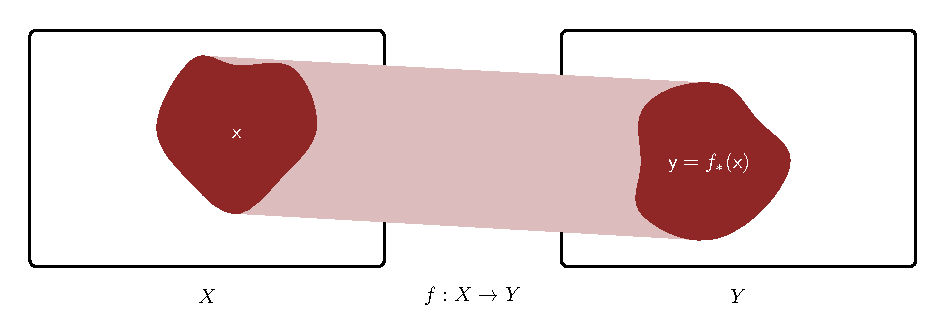
\includegraphics{figures/set_transformations/set_pushforward/set_pushforward.pdf}

}

}

\subcaption{\label{fig-set-pushforward}}
\end{minipage}%
%
\begin{minipage}[t]{0.10\linewidth}

{\centering 

~

}

\end{minipage}%
\newline
\begin{minipage}[t]{0.10\linewidth}

{\centering 

~

}

\end{minipage}%
%
\begin{minipage}[t]{0.80\linewidth}

{\centering 

\raisebox{-\height}{

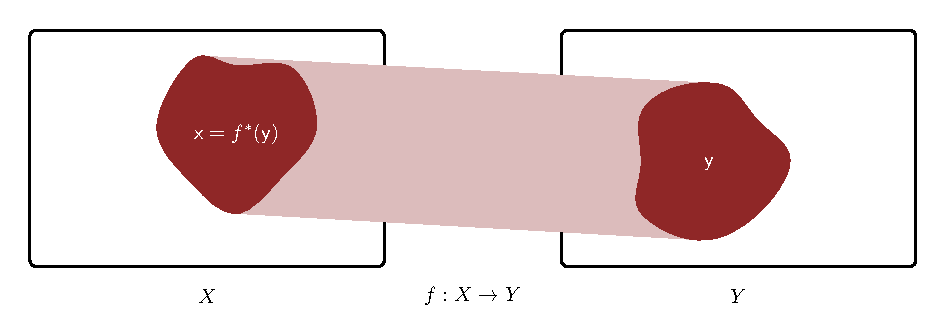
\includegraphics{figures/set_transformations/set_pullback/set_pullback.pdf}

}

}

\subcaption{\label{fig-set-pullback}}
\end{minipage}%
%
\begin{minipage}[t]{0.10\linewidth}

{\centering 

~

}

\end{minipage}%

\caption{\label{fig-set-transformations}Transformations of a set induce
transformations of subsets. (a) Subsets of the input space
\(\mathsf{x} \subset X\) can be pushed forward into subsets of the
output space, \(f_{*}(\mathsf{x}) \subset Y\). (b) Similarly subsets of
the output space \(\mathsf{y} \subset Y\) can be pullsed back into
subsets of the input space, \(f^{*}(\mathsf{y})\subset X\).}

\end{figure}

There is an asymmetry between these two induced transformations,
however, when we consider set operations. Both the pushforward and
pullback set maps are compatible with the union operation,
\begin{align*}
f_{*}(\cup_{i} \mathsf{x}) &= \cup_{i} f_{*}(\mathsf{x})
\\
f^{*}(\cup_{i} \mathsf{y}) &= \cup_{i} f^{*}(\mathsf{y}),
\end{align*} but only the pullback map is always compatible with the
intersection operation, \[
f^{*}(\cap_{i} \mathsf{y}) = \cap_{i} f^{*}(\mathsf{y}).
\] In general the intersection of any collection of input subsets pushes
forward to a \emph{subset} of the intersection of the individual
pushforward subsets (Figure~\ref{fig-set-op-consistency}). \[
f_{*}(\cup_{i} \mathsf{x}) \subseteq \cup_{i} f_{*}(\mathsf{x}).
\]

\begin{figure}

\begin{minipage}[t]{0.18\linewidth}

{\centering 

~

}

\end{minipage}%
%
\begin{minipage}[t]{0.64\linewidth}

{\centering 

\raisebox{-\height}{

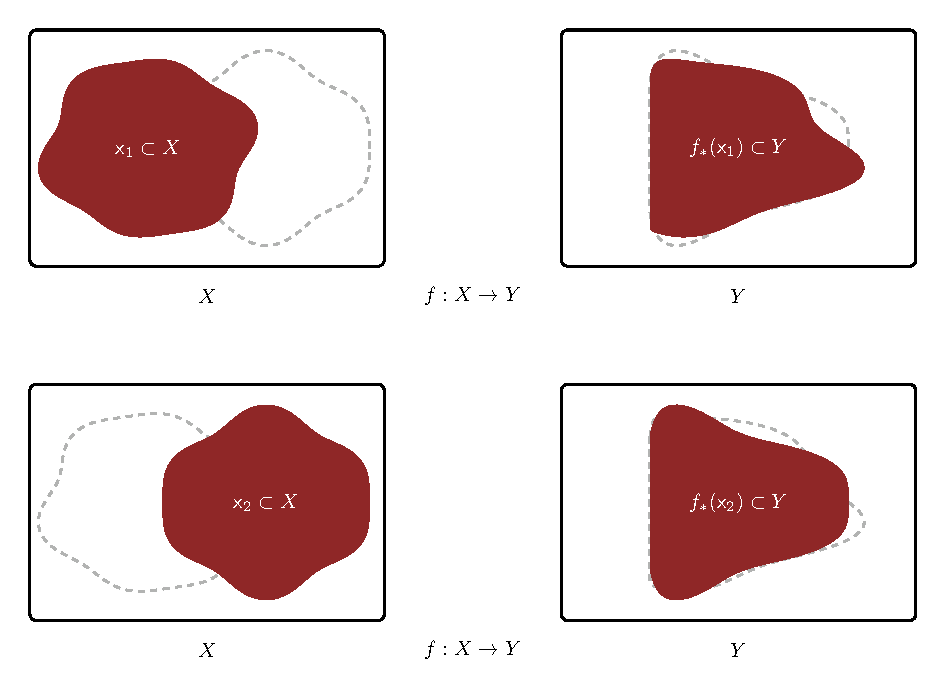
\includegraphics{figures/binary_op_consistency/inputs/inputs.pdf}

}

}

\subcaption{\label{fig-set-op-inputs}}
\end{minipage}%
%
\begin{minipage}[t]{0.18\linewidth}

{\centering 

~

}

\end{minipage}%
\newline
\begin{minipage}[t]{0.18\linewidth}

{\centering 

~

}

\end{minipage}%
%
\begin{minipage}[t]{0.64\linewidth}

{\centering 

\raisebox{-\height}{

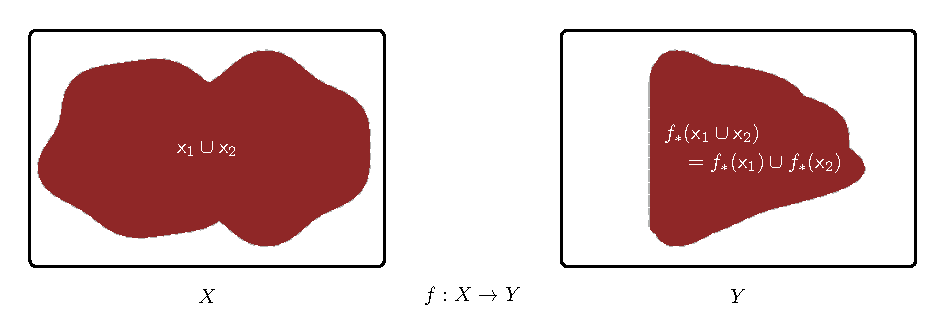
\includegraphics{figures/binary_op_consistency/union_pushforward/union_pushforward.pdf}

}

}

\subcaption{\label{fig-union-pushforward}}
\end{minipage}%
%
\begin{minipage}[t]{0.18\linewidth}

{\centering 

~

}

\end{minipage}%
\newline
\begin{minipage}[t]{0.18\linewidth}

{\centering 

~

}

\end{minipage}%
%
\begin{minipage}[t]{0.64\linewidth}

{\centering 

\raisebox{-\height}{

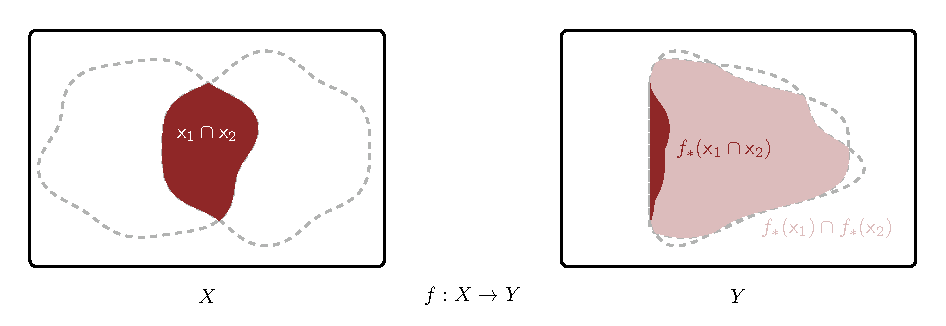
\includegraphics{figures/binary_op_consistency/intersection_pushforward/intersection_pushforward.pdf}

}

}

\subcaption{\label{fig-intersection-pushforward}}
\end{minipage}%
%
\begin{minipage}[t]{0.18\linewidth}

{\centering 

~

}

\end{minipage}%

\caption{\label{fig-set-op-consistency}In general (a) subset
pushforwards are not consistent with all of the binary set operations.
(b) The union of the pushforwards of two input subsets is always the
same as the pushforward of the union of the input subsets. (c) On the
other hand the intersection of the pushforwards of two input subsets is
in generally only a subset of the pushforward of the intersection of the
two input subsets. In other words the pushforward operation commutes
with the union operator, so that we can apply them in either order and
achieve the same result, but the pushforward operation does not commute
with the intersection operator. The pullback operation, however,
commutes with both the union and intersection operators.}

\end{figure}

This has an immediate consequence for \(\sigma\)-algebras: the
pushforward of an intersection of measurable input subsets isn't
necessarily a measurable output subset. Consequently a
\(\sigma\)-algebra of measurable subsets on \(X\) doesn't always push
forward into a \(\sigma\)-algebra of measurable subsets on \(Y\).

On the other hand a \(\sigma\)-algebra on \(Y\) \emph{does} always pull
back to a well-behaved \(\sigma\)-algebra on \(X\). If \(\mathcal{Y}\)
is a \(\sigma\)-algebra on \(Y\) then \[
f^{*} \mathcal{Y} =
\{ f^{*}(\mathsf{y}) \mid \mathsf{y} \in \mathcal{Y} \}
\] is referred to as the \textbf{pullback \(\sigma\)-algebra along
\(f\)} or the \textbf{\(\sigma\)-algebra generated by \(f\)}.

In order for a function \(f: X \rightarrow Y\) to preserve the structure
of two measurable spaces \((X, \mathcal{X})\) and \((Y, \mathcal{Y})\),
every measurable subset \(\mathsf{y} \in \mathcal{Y}\) needs to pull
back to a measurable subset in \(\mathcal{X}\), \[
f^{*}(\mathsf{y}) \in \mathcal{X},
\] Equivalently \(f\) preserves measurable structure only when \[
f^{*} \mathcal{Y} \subseteq \mathcal{X}.
\] Note that this does not require that \emph{every} measurable subset
\(\mathsf{x} \in \mathcal{X}\) pushes forward to a measurable subset in
\(\mathcal{Y}\); we can safely ignore measurable input subsets without
compromising the \(\sigma\)-algebra on the output space.

Functions that preserve measurable structure are known as
\textbf{\((\mathcal{X}, \mathcal{Y})\)-measurable functions}. When the
\(\sigma\)-algebras on the input and output space are unambiguous this
is often shortened to just \textbf{measurable functions}. I will also
use the more compact notation \[
f : (X, \mathcal{X}) \rightarrow (Y, \mathcal{Y})
\] to denote \((\mathcal{X}, \mathcal{Y})\)-measurable functions.

We've already encountered measurable functions in
\href{https://betanalpha.github.io/assets/chapters_html/expectation_values.html}{Chapter
5} when introducing measure-informed integration. A real-valued function
\(f : X \rightarrow \mathbb{R}\) can be integrated on the measure space
\((X, \mathcal{X}, \mu)\) if every half-open interval on the output
space pulls back to a measurable subset on the input space, \[
f^{*}( \, (-\infty, x) \, ) \in \mathcal{X}.
\] This condition, however, is equivalent to every subset in the Borel
\(\sigma\)-algebra of the real line,
\(\mathsf{y} \in \mathcal{B}_{\mathbb{R}}\), pulling back to a
measurable subset on the input space, \[
f^{*}( \mathsf{y} ) \in \mathcal{X}.
\]

In other words what we referred to as ``\(\mathcal{X}\)-measurable
real-valued functions'' in
\href{https://betanalpha.github.io/assets/chapters_html/expectation_values.html}{Chapter
5} are more formally
\((\mathcal{X}, \mathcal{B}_{\mathbb{R}})\)-measurable functions. The
former notation takes the Borel \(\sigma\)-algebra on the real line for
granted, while the latter makes it more explicit. This is a common
shorthand -- references to ``measurable functions'' without any
specification almost always imply Borel \(\sigma\)-algebras on the input
and output spaces.

Fortunately this shorthand isn't too problematic in practice because we
will almost always be working with measures defined over Borel
\(\sigma\)-algebras derived from the topological structure of the
relevant spaces. Consequently a function \(f : X \rightarrow Y\) mapping
the Borel measurable space \((X, \mathcal{B}_{X})\) into the Borel
measurable space \((Y, \mathcal{B}_{Y})\) might be described as
\((\mathcal{B}_{X}, \mathcal{B}_{Y})\)-measurable, \textbf{Borel
measurable}, or even just ``measurable''.

Continuous functions that respect the topological structure of the input
and outputs spaces are always Borel measurable, but so too are functions
that are only piece-wise continuous. Ultimately Borel measurability is a
much weaker condition than topological continuity because we can map
open subsets in the output space into not only open subsets in the
output space, but also closed subsets in the output space and even any
subset that we can derive from unions and intersections of open and
closed subsets in the input space.

\begin{figure}

{\centering 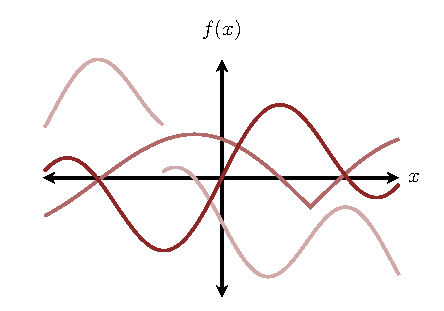
\includegraphics[width=0.6\textwidth,height=\textheight]{figures/measurable_functions/measurable_functions.pdf}

}

\caption{\label{fig-label}Most of the functions that we encounter in
practice are measurable with respect to the standard
\(\sigma\)-algebras. For example functions
\(f: \mathbb{R} \rightarrow \mathbb{R}\) that are smooth,
non-differentiable but continuous, and even discontinuous at a countable
number of points are all
\((\mathcal{B}_{\mathbb{R}}, \mathcal{B}_{\mathbb{R}})\)-measurable.}

\end{figure}

When working with finite-dimensional spaces in practice it is safe to
assume that not only all but the most pathological subsets are
measurable but also that all but the most pathological functions are
measurable. Infinite-dimensional spaces are another matter, but that
those spaces will largely be outside of the scope of this book.

\hypertarget{transforming-measures}{%
\section{Transforming Measures}\label{transforming-measures}}

Conveniently the pullback of measurable subsets allows us to pushforward
measures from the input space to a compatible measure on the output
space. Given a \((\mathcal{X}, \mathcal{Y})\)-measurable function
\(f : X \rightarrow Y\) any measure
\(\mu : \mathcal{X} \rightarrow [0, \infty]\) defines a
\textbf{pushforward measure} by the allocations \begin{alignat*}{6}
f_{*} \mu :\; & \mathcal{Y} & &\rightarrow& \; & \mathbb{R}^{+} &
\\
& \mathsf{y} & &\mapsto& &
f_{*} \mu (\mathsf{y}) = \mu(f^{*}(\mathsf{y})) &.
\end{alignat*} In words the pushforward measure allocated to any
measurable subset on the output space \(\mathsf{y} \in \mathcal{Y}\) is
computed by pulling the subset back to the input space
\(f^{*}(\mathsf{y}) \in \mathcal{X}\) and then evaluating the initial
measure, \(\mu(f^{*}(\mathsf{y}))\)
(Figure~\ref{fig-pushforward-measure}).

\begin{figure}

{\centering 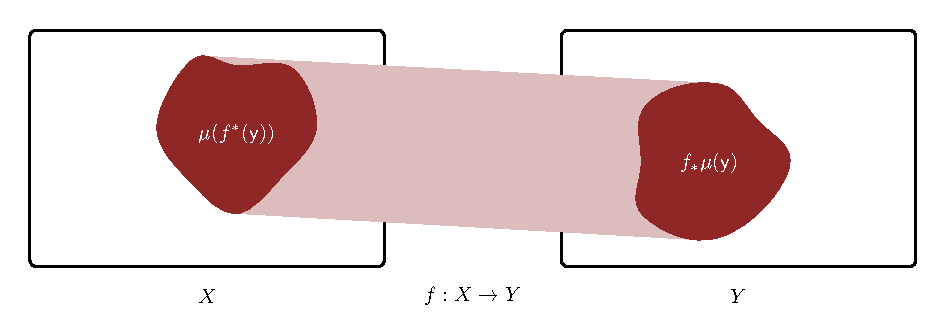
\includegraphics[width=0.8\textwidth,height=\textheight]{figures/pushforward_measure/pushforward_measure.pdf}

}

\caption{\label{fig-pushforward-measure}Because measurable output
subsets pullback to measurable input subsets along measurable functions
we can push forward measure allocations. In particular the pushforward
measure allocated to the measurable output subset
\(\mathsf{y} \in \mathcal{Y}\) is given by pulling it back to the input
space, \(f^{*}(\mathsf{y}) \in \mathcal{X}\), and then querying the
initial measure, \(\mu(f^{*}(\mathsf{y}))\).}

\end{figure}

The exact interpretation of a pushforward measure will depend on the
interpretation of the input measure and the transformation. Consider,
for example, a probability distribution \(\pi\) defined on the input
space that we interpret as quantifying uncertainty. This probability
distribution captures our uncertainty about the \emph{inputs} to a
function \(f\) while the pushforward probability distribution
\(f_{*} \pi\) quantifies the corresponding uncertainty in the
\emph{output} of the function. In other words the pushforward
transformation \emph{propagates} the initial uncertainty through the
deterministic mapping.

At the same time certain functions can endow the corresponding
pushforward measures with particular interpretations.

\hypertarget{sec:terminology}{%
\subsection{Pushforward Terminology}\label{sec:terminology}}

Pushforward measures are ubiquitous in applied probability theory,
although they are often better known by other names.

For example consider a finite input space \(X\), \[
X = \{ \blacksquare, \clubsuit, \bigcirc,
       \diamondsuit, \triangle, \bowtie \},
\] a finite output space \(Y\), \[
Y = \{ \heartsuit, \spadesuit, \bigstar \},
\] and a function \(f : X \rightarrow Y\) defined by the relations
(Figure~\ref{fig-finite-marginal-function}) \begin{align*}
f(\blacksquare) &= \spadesuit
\\
f(\clubsuit) &= \heartsuit
\\
f(\bigcirc) &= \bigstar
\\
f(\diamondsuit) &= \spadesuit
\\
f(\triangle) &= \heartsuit
\\
f(\bowtie) &= \spadesuit
\end{align*}

These relationships between input and output points become particularly
well-organized when we arrange the input elements into a table, with
each row collecting all of the input elements that map to a particular
output element (Figure~\ref{fig-finite-marginal-table}). Conveniently
the pushforward measure allocated to each output atomic subset is then
given by summing the input atomic subset allocations in each the
corresponding row (Figure~\ref{fig-finite-marginal-initial-allocations},
Figure~\ref{fig-finite-marginal-initial-allocations}). In other words
the pushforward allocations fit nicely into the \emph{margins} of the
table.

\begin{figure}

\begin{minipage}[t]{\linewidth}

{\centering 

\raisebox{-\height}{

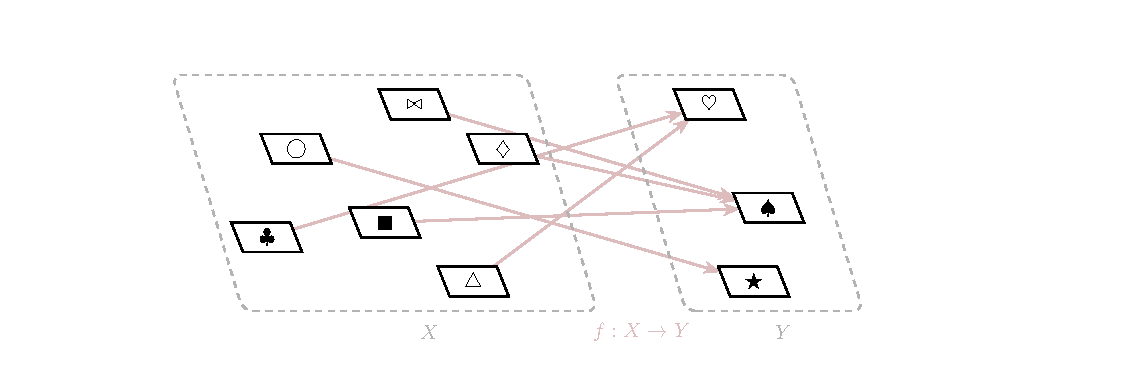
\includegraphics{figures/finite_marginal/function/function.pdf}

}

}

\subcaption{\label{fig-finite-marginal-function}}
\end{minipage}%
\newline
\begin{minipage}[t]{\linewidth}

{\centering 

\raisebox{-\height}{

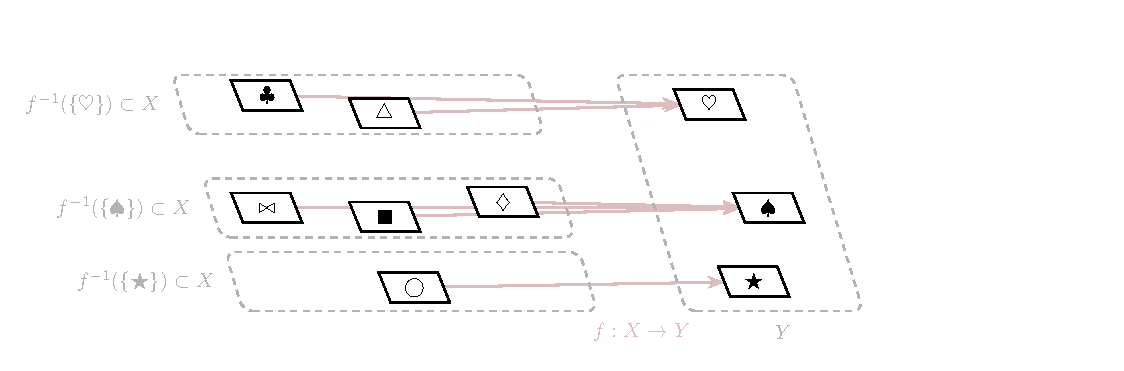
\includegraphics{figures/finite_marginal/table/table.pdf}

}

}

\subcaption{\label{fig-finite-marginal-table}}
\end{minipage}%
\newline
\begin{minipage}[t]{\linewidth}

{\centering 

\raisebox{-\height}{

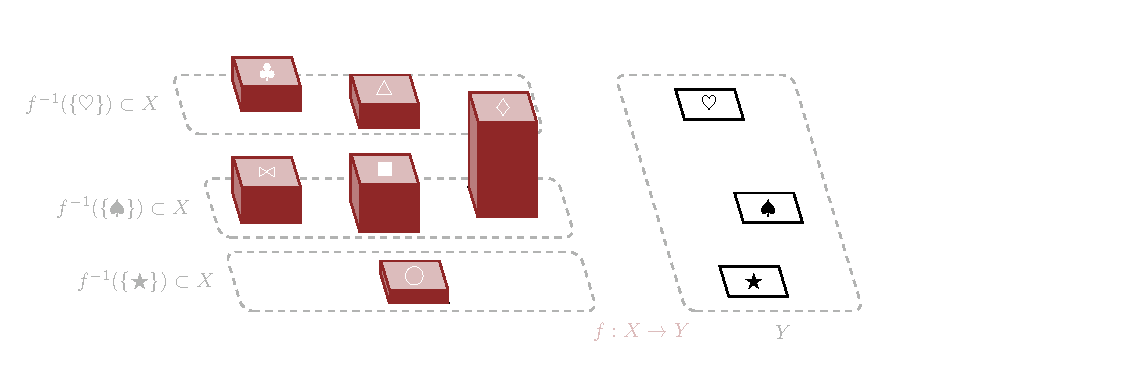
\includegraphics{figures/finite_marginal/initial_allocations/initial_allocations.pdf}

}

}

\subcaption{\label{fig-finite-marginal-initial-allocations}}
\end{minipage}%
\newline
\begin{minipage}[t]{\linewidth}

{\centering 

\raisebox{-\height}{

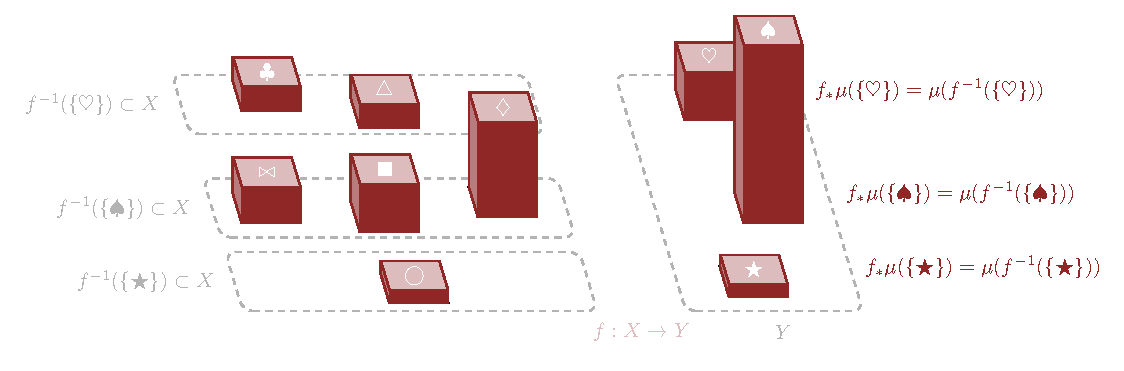
\includegraphics{figures/finite_marginal/marginal_allocations/marginal_allocations.pdf}

}

}

\subcaption{\label{fig-finite-marginal-marginal-allocations}}
\end{minipage}%

\caption{\label{fig-finite-marginal}On finite spaces (a) functions
\(f: X \rightarrow Y\) (b) are naturally organized into tables, with
each row collecting all of the input points that map to each output
point. (c) Given an input measure \(\mu\) (d) we can compute the
pushforward measure allocations by summing the \(\mu\) allocations in
each row and then displaying the results in the margins of the table.}

\end{figure}

Historically these kinds of graphical organizations motivated the term
\textbf{marginal measure} to describe pushforward measures, or
\textbf{marginal probability distribution} in the case of an input
probability distribution. Today this terminology is common even when the
input and output spaces are not finite, and the tabular representation
of functions isn't quite as useful
(Figure~\ref{fig-continuous-marginal}).

\begin{figure}

\begin{minipage}[t]{0.02\linewidth}

{\centering 

~

}

\end{minipage}%
%
\begin{minipage}[t]{0.32\linewidth}

{\centering 

\raisebox{-\height}{

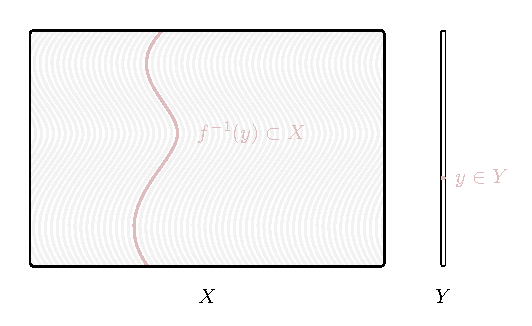
\includegraphics{figures/continuous_marginal/level_sets/level_sets.pdf}

}

}

\subcaption{\label{fig-level-sets}}
\end{minipage}%
%
\begin{minipage}[t]{0.32\linewidth}

{\centering 

\raisebox{-\height}{

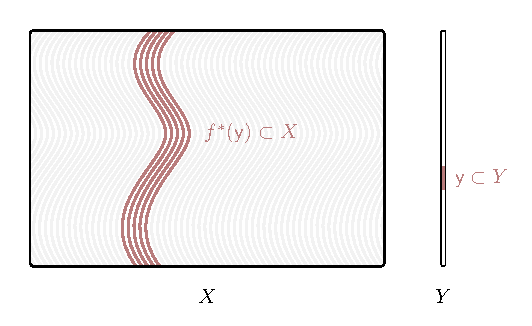
\includegraphics{figures/continuous_marginal/pullback_sets/pullback_sets.pdf}

}

}

\subcaption{\label{fig-pullback-sets}}
\end{minipage}%
%
\begin{minipage}[t]{0.32\linewidth}

{\centering 

\raisebox{-\height}{

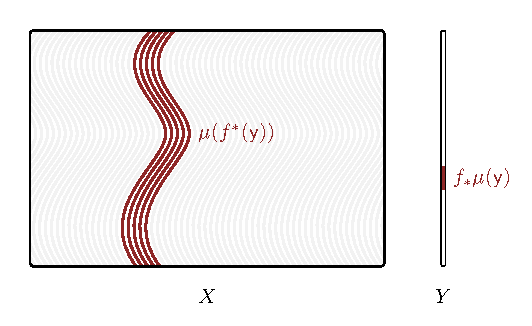
\includegraphics{figures/continuous_marginal/marginal_probability/marginal_probability.pdf}

}

}

\subcaption{\label{fig-marginal-probability}}
\end{minipage}%
%
\begin{minipage}[t]{0.02\linewidth}

{\centering 

~

}

\end{minipage}%

\caption{\label{fig-continuous-marginal}When working on general spaces
the tabular organization of a function \(f: X \rightarrow Y\)
generalizes to (a) collections of level sets \(f^{-1}(y) \subset X\),
one for each output point \(y \in Y\). (b) The pullback of any output
subset is the union of these level sets and (c) the pushforward measure
allocated to any output subset is effectively the sum of the measures
allocated to the relevant level sets. These pushforward allocations can
then be informally collected into the ``margins''.}

\end{figure}

Another popular naming convention arises when the output space is a
subset of the input space, \(Y \subset X\). In this case a function
\(f: X \rightarrow Y\) \textbf{projects} the input space onto the output
subset (Figure~\ref{fig-projection}). Pushing forward measures along
this projection \emph{collapses} the total measure allocated to the
input space into the smaller output space.

\begin{figure}

\begin{minipage}[t]{0.20\linewidth}

{\centering 

~

}

\end{minipage}%
%
\begin{minipage}[t]{0.30\linewidth}

{\centering 

\raisebox{-\height}{

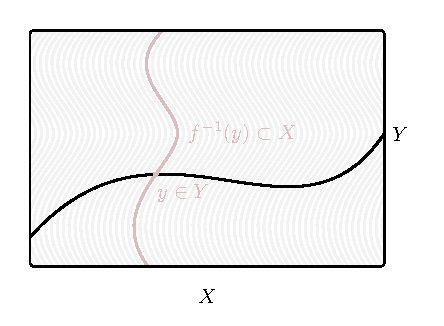
\includegraphics{figures/projection/level_sets/level_sets.pdf}

}

}

\subcaption{\label{fig-level-sets}}
\end{minipage}%
%
\begin{minipage}[t]{0.30\linewidth}

{\centering 

\raisebox{-\height}{

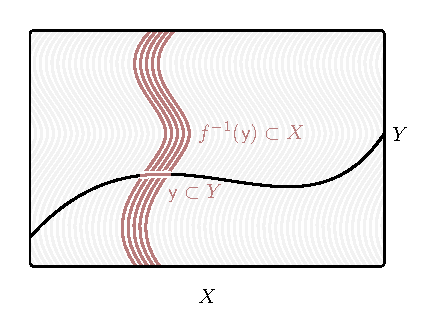
\includegraphics{figures/projection/pullback_sets/pullback_sets.pdf}

}

}

\subcaption{\label{fig-pullback-sets}}
\end{minipage}%
%
\begin{minipage}[t]{0.20\linewidth}

{\centering 

~

}

\end{minipage}%
\newline
\begin{minipage}[t]{0.05\linewidth}

{\centering 

~

}

\end{minipage}%
%
\begin{minipage}[t]{0.90\linewidth}

{\centering 

\raisebox{-\height}{

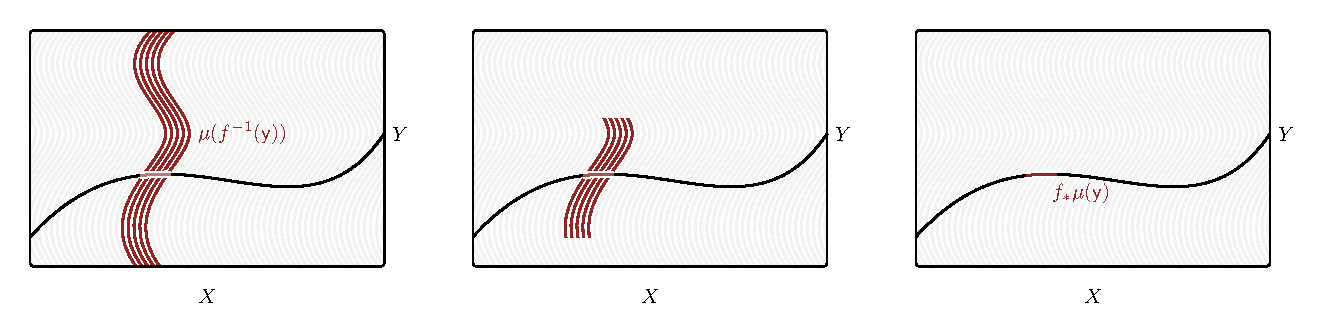
\includegraphics{figures/projection/marginal_probability/marginal_probability.pdf}

}

}

\subcaption{\label{fig-marginal-probability}}
\end{minipage}%
%
\begin{minipage}[t]{0.05\linewidth}

{\centering 

~

}

\end{minipage}%

\caption{\label{fig-projection}When a function \(f: X \rightarrow Y\)
maps an input space into a subset of itself, \(Y \subset X\), then
pushforward measures can be interpreted as projections of the initial
measure. (a) In this case each level set \(f^{-1}(y)\) is anchored to a
point \(y \in X\) and (b) the pullback of an output subset is anchored
to the points in that subset. (c) The pushforward measure collapsed the
measure allocated to each level set down to the corresopnding anchor
point.}

\end{figure}

Consider for example the unit interval interpreted as a subset of a real
line, \[
(0, 1) \subset R.
\] One way to squeeze the entire real line into \((0, 1)\) is to apply
the \textbf{logistic function}, \begin{alignat*}{6}
\mathrm{logistic} :\; & \mathbb{R} & &\rightarrow& \; & (0, 1) &
\\
& x & &\mapsto& & \frac{1}{1 + \exp(-x)}  &.
\end{alignat*}

The logistic function preserves topological structure, pushing open
intervals in \(\mathbb{R}\) forward into open intervals in \((0, 1)\),
\[
\mathrm{logistic}_{*}( \, (x_{1}, x_{2}) \, )
=
( \, \mathrm{logistic}(x_{1}), \mathrm{logistic}(x_{2}) \, ).
\] At the same time open intervals in \((0, 1)\) are pulled back into
open intervals in \(\mathbb{R}\), \[
\mathrm{logistic}^{*}( \, (y_{1}, y_{2}) \, )
=
( \, \mathrm{logistic}^{-1}(y_{1}), \mathrm{logistic}^{-1}(y_{2}) \, ).
\] Consequently the logistic function is Borel measurable.

When pushing forward measures along the logistic function the measure
allocated to any open interval is squeezed into a narrower interval,
\begin{align*}
\mu_{*}( \, (y_{1}, y_{2}) \, )
&=
\mu( \, \mathrm{logistic}^{*}( \, (y_{1}, y_{2}) \, ) \, )
\\
&=
\mu( \, (\, \mathrm{logistic}^{-1}(y_{1}),
            \mathrm{logistic}^{-1}(y_{2}) \, ) \, ).
\end{align*}

\begin{figure}

{\centering 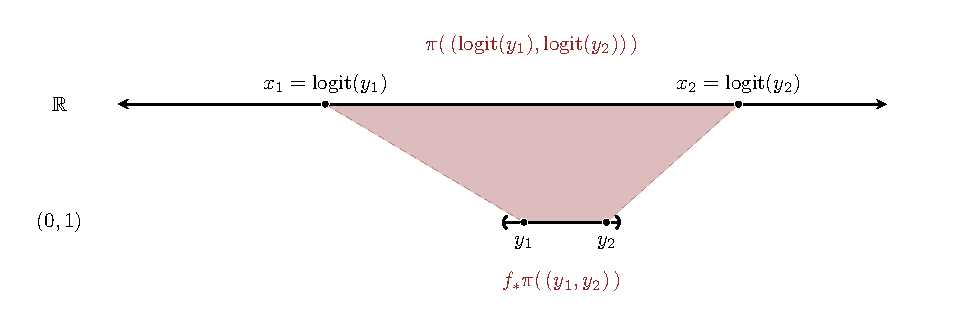
\includegraphics[width=0.95\textwidth,height=\textheight]{figures/line_to_interval/line_to_interval.pdf}

}

\caption{\label{fig-line-to-interval}The logistic function squeeze an
entire real line into the unit interval. When we push an input measure
forward along the logistic function the measure allocated to an input
intervals is squeezed into a narrow interval.}

\end{figure}

\hypertarget{lossy-pushforward-measures}{%
\subsection{Lossy Pushforward
Measures}\label{lossy-pushforward-measures}}

We can always push measures forward along measurable functions, but in
general we cannot pull them back. This asymmetry arises because the
pushforward operation can \emph{lose information}.

Consider the function between finite spaces that we introduced in
\href{@sec:terminology}{Section 2.1}. A measure \(\mu\) on the input
space defines the pushforward atomic allocation \begin{align*}
f_{*} \mu( \{ \heartsuit \} )
&=
\mu( f^{*}(\heartsuit) )
\\
&=
\mu( \{ \clubsuit, \triangle \} )
\\
&=
\mu( \{ \clubsuit \} ) + \mu( \{ \triangle \} ).
\end{align*} Because input elements \(\clubsuit\) and \(\triangle\) map
to the same output element their atomic allocations are combined into a
single pushforward atomic allocation.

If we are given only the pushforward allocation
\(f_{*} \mu( \{ \heartsuit \} )\) then we will not have enough
information to fully recover the initial allocations
\(\mu( \{ \triangle \} )\) and \(\mu( \{ \triangle \} )\). We can
constrain their sum, \[
f_{*} \mu( \{ \heartsuit \} )
=
\mu( \{ \clubsuit \} ) + \mu( \{ \triangle \} ),
\] but there are infinitely many input measures consistent with such a
constraint.

For a more sophisticated example let's investigate a function that maps
a real line into integers by rounding each real number to the next
largest integer, \begin{alignat*}{6}
f :\; & \mathbb{R} & &\rightarrow& \; & \mathbb{Z} &
\\
& x & &\mapsto& & \lceil x \rceil  &.
\end{alignat*} This function collapses every point in the half-open
interval \((n - 1, n]\) to the integer \(n\) so that the atomic subsets
on the output space pull back to those input intervals
(Figure~\ref{fig-line-to-integers}), \[
f^{*}( \{ n \} ) = (n - 1, n].
\]

\begin{figure}

{\centering 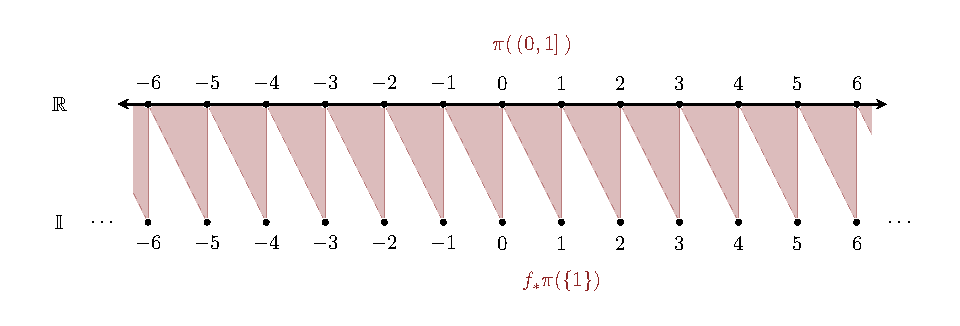
\includegraphics[width=0.95\textwidth,height=\textheight]{figures/line_to_integers/line_to_integers.pdf}

}

\caption{\label{fig-line-to-integers}Rounding real numbers to the
next-largest integer defines a map from a real line to the integers.
Input measure allocated to the half-open intervals \((n - 1, n]\)
projects down to the corresponding integer \(n\).}

\end{figure}

Along \(f\) the Lebesgue measure on the real line pushes forward to a
measure on the integers with the atomic allocations \begin{align*}
f_{*} \lambda( \{ n \} )
&=
\lambda( f^{*} ( \{ n \} ) )
\\
&=
\lambda( \, (n, n - 1] \, )
\\
&=
n - (n - 1)
\\
&=
1.
\end{align*} In other words the pushforward of the Lebesgue measure
along this rounding map is just the counting measure!

The counting measure on the output space, however, does not provide any
information about how to distribute the atomic allocation
\(\chi( \{ n \} ) = 1\) across the entire pullback subset
\((n - 1, n]\). Instead there are an infinite numbers of ways that the
measure \(\chi( \{ n \} ) = 1\) could be consistently reallocated across
\((n - 1, n]\) and we have no criteria for preferring one over another.

\hypertarget{lossless-pushforward-measures}{%
\subsection{Lossless Pushforward
Measures}\label{lossless-pushforward-measures}}

Because most pushforward measures lose information about the initial
allocations the exceptional measures that preserve information are
particulary notable.

As we saw in \href{@sec:pushforward-sets}{Section 1} pushforward sets do
not generally respect the intersection set operator, preventing us from
pushing forward \(\sigma\)-algebras from the input space to the output
space. Pushing sets forward along injective functions, however, does
respect the intersection operator. Consequently we can always push
forward \(\sigma\)-algebras along injective functions.

When working with measurable spaces that are already equipped with
\(\sigma\)-algebras, \((X, \mathcal{X})\) and \((Y, \mathcal{Y})\) any
injective function \(f : X \rightarrow Y\) that both pulls back
measurable output subsets to measurable input subsets, \[
f^{*}(\mathsf{y}) \subset \mathcal{X},
\] \emph{and} pushes forward measurable input subsets to measurable
output subsets, \[
f_{*}(\mathsf{x}) \subset \mathcal{Y}.
\] is said to be \textbf{\(( \mathcal{X}, \mathcal{Y} )\)-bimeasurable},
or simply \textbf{bimeasurable} when the \(\sigma\)-algebras are
unambiguous.

Because the pushforward and pullback maps along injective functions
always satisfy \[
f^{*} \circ f_{*} = I
\] we also have \[
f^{*}(\mathcal{Y}) = \mathcal{X}.
\] In other words the \(\sigma\)-algebra generated by a bimeasurable
function is just the input \(\sigma\)-algebra.

As with measurable functions, bimeasurable functions allow us to push
forward any measure on the input space
\(\mu : \mathcal{X} \rightarrow [0, \infty]\) to a corresponding measure
on the output space \(\mu_{*} : \mathcal{Y} \rightarrow [0, \infty]\)
with the allocations \[
\mu_{*}(\mathsf{y}) = \mu( \, f^{*}(\mathsf{y}) \, ).
\] Bimeasurable functions also allow us to pull back any measure
\(\nu : \mathcal{Y} \rightarrow [0, \infty]\) on the output space to a
corresponding measure \(\nu^{*} : \mathcal{X} \rightarrow [0, \infty]\)
on the input space with the allocations \[
\nu^{*}(\mathsf{x}) = \nu( \, f_{*}(\mathsf{x}) \, ).
\]

When a function \(f : (X, \mathcal{X}) \rightarrow (Y, \mathcal{Y})\) is
not only bimeasurable by also bijective then these operations are
consistent with each other. Pulling back a pushforward measure always
recovers the input allocations, \begin{align*}
f^{*} \mu_{*} (\mathsf{x})
&=
\mu^{*}( \, f_{*}(\mathsf{x}) \, )
\\
&=
\mu( \, f^{*} \circ f_{*}(\mathsf{x}) \, )
\\
&=
\mu( \mathsf{x} ),
\end{align*} and pushing forward a pullback measure always recovers the
output allocations, \begin{align*}
f_{*} \nu^{*} (\mathsf{y})
&=
\nu^{*}( \, f^{*}(\mathsf{y}) \, )
\\
&=
\nu( \, f_{*} \circ f^{*}(\mathsf{y}) \, )
\\
&=
\nu( \mathsf{y} ).
\end{align*} In other words we can completely reconstruct any input
measure from its pushforward allocations and any output measure from its
pullback allocations. Bimeasurable functions do not lose information!

Two measure spaces \((X, \mathcal{X}, \mu)\) and
\((Y, \mathcal{Y}, \nu)\) that are related by a bimeasurable function
\(f : X \rightarrow Y\) provide equivalent measure-theoretic
information, \begin{align*}
f_{*} \mu &= \nu
\\
f^{*} \nu &= \mu.
\end{align*} Because they quantify the same information they can be
interpreted as different mathematical \emph{representations} of a
common, abstract measure system.

For example because every permutation of a countable set preserves the
discrete \(\sigma\)-algebra every permutation of a countable set is a
bimeasurable bijection, transforming any discrete measure into another,
equivalent discrete measure. In practice this means that we are free to
choose the permutation that yields the most convenient organization of
the underlying set without having to worry about compromising the
information encoded in the original space!

Similarly every continuous bijection between two real lines is
bimeasurable with respect to the Borel \(\sigma\)-algebras. Continuous
bijections then allow us to transform a measure over a rigid real line
into a measure on another rigid real line without losing information.
Equivalently these maps allow us to transform a measure over any
parameterization of a flexible real line into a measure over any other
parameterization of that space without losing any resolution of the
system. This gives us the freedom to choose the units or coordinate
system that are most convenient in a given application without having to
worry about affecting the measure structure.

\hypertarget{sec:transforming-integrals}{%
\section{Transforming Measure-Informed
Integrals}\label{sec:transforming-integrals}}

Once we know how to transform subset allocations we can, at least in
theory, define integrals with respect to a pushforward measure on the
output space and relate them to integrals with respect to the initial
measure on the input space. Fortunately that relationship ends up being
relatively straightforward.

Given a function \(\phi : X \rightarrow Y\) any real-valued function on
the output space \(f : Y \rightarrow \mathbb{R}\) pulls back to a
real-valued function on the input space
\(\phi^{*} f : X \rightarrow \mathbb{R}\) by composition, \[
\phi^{*} f(x) = f \circ \phi (x) = f(\phi(x)).
\] Additionally if \(\phi : X \rightarrow Y\) is a
\((\mathcal{X}, \mathcal{Y})\)-measurable function and
\(f : Y \rightarrow \mathbb{R}\) is a
\((\mathcal{Y}, \mathbb{B}_{\mathbb{R}})\)-measurable function then
\(\phi^{*} f = f \circ \phi\) will always be a
\((\mathcal{X}, \mathbb{B}_{\mathbb{R}})\)-measurable function. In other
words integrands on the output space always pullback to integrands on
the input space along measurable transformations.

When the input space is endowed with a measure \(\mu\), and the output
space is endowed with the pushforward measure \(\phi_{*} \mu\), we can
use these two integrands to define two measure-informed integrals: one
on the input space, \[
\mathbb{I}_{\mu} [ \phi^{*} f ],
\] and one on the output space, \[
\mathbb{I}_{\phi_{*} \mu} [ f ].
\] Conveniently these measure-informed integrals are always equal, \[
\mathbb{I}_{\mu} [ \phi^{*} f ] = \mathbb{I}_{\phi_{*} \mu} [ f ].
\] When we're working with probability distributions this becomes a
relationship between equivalent expectation values, \[
\mathbb{E}_{\pi} [ \phi^{*} f ]
=
\mathbb{E}_{\phi^{*} \pi} [ f ].
\]

This equality means that we never have to explicitly construct a
pushforward measure in practice. We can compute any integral with
respect to \(\phi_{*} \mu\) by pulling back the output integrand to the
input space, \[
\phi^{*} f = f \circ \phi,
\] and integrating with respect to \(\mu\). So long as we know how to
compute \(\mu\)-informed integrals we can compute
\(\phi_{*} \mu\)-informed integrals.

While we're on the topic of measure-informed integration, notice that we
have two ways for a measure space \((X, \mathcal{X}, \mu)\) to consume a
function
\(f : (X, \mathcal{X}) \rightarrow  (\mathbb{R}, \mathcal{B}_{\mathbb{R}})\).
So long as \(f\) is \(\mu\)-integrable we can integrate \(f\) with
respect to \(\mu\) to give the single real number
\(\mathbb{I}_{\mu}[f] \in \mathbb{R}\). On the other hand we can also
push \(\mu\) forward along \(f\) to construct an entire measure
\(f_{*} \mu\) over the possible output values!

The mean of the pushforward measure \(f_{*} \mu\) is given by
\begin{align*}
\mathbb{M}_{f^{*} \mu}
&=
\mathbb{I}_{f^{*} \mu} [ \iota ]
\\
&=
\mathbb{I}_{\mu} [ \iota \circ f ]
\\
&=
\mathbb{I}_{\mu} [ f ].
\end{align*} In other words the \(\mu\)-informed integral of \(f\) is
always equal to the mean of the corresponding pushforward measure!

Because of this concurrence the \(\mu\)-informed integral of a function
is sometimes referred to as ``the mean of \(f\)''. Similarly the
\(\mu\)-informed integral of \begin{align*}
\mathbb{I}_{f^{*} \mu} [ (\iota - \mathbb{M}_{f^{*} \mu})^{2} ]
&=
\mathbb{I}_{\mu} [ (\iota \circ f - \mathbb{M}_{f^{*} \mu})^{2} ]
\\
&=
\mathbb{I}_{\mu} [ (f - \mathbb{M}_{f^{*} \mu})^{2} ]
\end{align*} is sometimes referred to as ``the variance of \(f\)''.

Personally I try to avoid this terminologies because I find that they
facilitate confusion between the two operations. I do not, however, shy
away from using certain \(\mu\)-informed integrals to quantify the
properties of a pushforward measure \(f_{*} \mu\). Indeed this is an
incredibly powerful tool in practice and one that we discuss more
thoroughly in \href{@sec:1d-pushforward-characterizations}{Section 5}.

\hypertarget{transforming-probability-density-functions}{%
\section{Transforming Probability Density
Functions}\label{transforming-probability-density-functions}}

In practice we rarely, if ever, define probability distributions with
subset allocations but rather rely on probability density functions with
respect to convenient reference measures. To transform probability
distributions in this applied context we will need to know how to push
forward probability density functions along measurable transformations.

\hypertarget{directly-transforming-probability-density-functions}{%
\subsection{Directly Transforming Probability Density
Functions}\label{directly-transforming-probability-density-functions}}

When an initial probability distribution \(\pi\) and reference measure
\(\nu\) are fixed the transformation properties of the corresponding
probability density function is straightforward to construct for
bijective functions.

On the input space we can define the probability density function \[
\frac{ \mathrm{d} \pi }{ \mathrm{d} \nu} : X \rightarrow \mathbb{R}^{+}.
\] At the same time given a function
\(f : (X, \mathcal{X}) \rightarrow (Y, \mathcal{Y})\) we can push
forward both \(\pi\) and \(\nu\) to measures on the output space and
construct the probability density function between them, \[
\frac{ \mathrm{d} f_{*} \pi }{ \mathrm{d} f_{*} \nu} :
Y \rightarrow \mathbb{R}^{+}.
\]

Because we're using a consistent reference measure these two functions
are related by composition, \[
\frac{ \mathrm{d} \pi }{ \mathrm{d} \nu}(x)
\overset{\nu}{=}
\frac{ \mathrm{d} f_{*} \pi }{ \mathrm{d} f_{*} \nu} \circ f(x).
\] In other words the output probability density function
\(\mathrm{d} f_{*} \pi / \mathrm{d} f_{*} \nu\) pulls back to the input
probability density function \(\mathrm{d} \pi / \mathrm{d} \nu\).

When \(f\) is a bijection we can use its inverse to construct an output
probability density function from an input probability density function,
\[
\frac{ \mathrm{d} f_{*} \pi }{ \mathrm{d} f_{*} \nu}(y)
\overset{f_{*} \nu}{=}
\frac{ \mathrm{d} \pi }{ \mathrm{d} \nu} \circ f^{-1}(y).
\]

In a practice, however, the pushforward of the initial reference measure
\(f_{*} \nu\) might not actually be the most convenient reference
measure on the output space. For example a uniform measure over the
input space will not generally push forward to a uniform measure over
the output space. If we want to construct probability density functions
on the output space relative to a \emph{different} reference measure
\(\lambda\) then the relevant probability density function we need is no
longer \[
\frac{ \mathrm{d} f_{*} \pi }{ \mathrm{d} f_{*} \nu} :
Y \rightarrow \mathbb{R}^{+}.
\] but rather \[
\frac{ \mathrm{d} f_{*} \pi }{ \mathrm{d} \lambda} :
Y \rightarrow \mathbb{R}^{+}.
\]

Fortunately we can still relate this output probability density function
to the initial probability density function with the Radon-Nikodym chain
rule. If \(f_{*} \nu\) is absolutely continuous with respect to
\(\lambda\) then we can expand the desired output probability density
function into \[
\frac{ \mathrm{d} f_{*} \pi }{ \mathrm{d} \lambda}(y)
\overset{\lambda}{=}
\frac{ \mathrm{d} f_{*} \pi }{ \mathrm{d} f_{*} \nu}(y)
\cdot
\frac{ \mathrm{d} f_{*} \pi }{ \mathrm{d} \lambda}(y).
\] When \(f\) is measurable \emph{and} bijective then we can derive the
first contribution from the initial probability density function and the
function inverse, \[
\frac{ \mathrm{d} f_{*} \pi }{ \mathrm{d} \lambda}(y)
\overset{\lambda}{=}
\frac{ \mathrm{d} \pi }{ \mathrm{d} \nu} \circ f^{-1}(y)
\cdot
\frac{ \mathrm{d} f_{*} \nu }{ \mathrm{d} \lambda}(y).
\]

The second term in this transformation formula, \[
\frac{ \mathrm{d} f_{*} \nu }{ \mathrm{d} \lambda}(y),
\] quantifies how \emph{warped} the pushforward reference measure
\(f_{*} \nu\) is relative to the desired reference measure \(\lambda\).
When \[
\frac{ \mathrm{d} f_{*} \nu }{ \mathrm{d} \lambda}(y)
\overset{\lambda}{=} 1
\] the two reference measures are equivalent and the transformation rule
reduces to our initial calculation.

Unfortunately this warping contribution is often difficult to compute,
limiting how often we can applying the transformation formula directly.
To compute it in practice we usually need to consider the transformation
properties of measure-informed integrals, \begin{align*}
\mathbb{I}_{\nu}[g \circ f]
&=
\mathbb{I}_{f_{*} \nu}[g]
\\
\mathbb{I}_{\nu} [ g \circ f ]
&=
\mathbb{I}_{\lambda} \left[
\frac{ \mathrm{d} f_{*} \nu }{ \mathrm{d} \lambda} \cdot g
\right].
\end{align*} If we can relate \(\nu\)-informed integration on the input
space to \(\lambda\)-informed integration out the output space then this
relationship may allow us to compute the warping factor
\(\mathrm{d} f_{*} \nu / \mathrm{d} \lambda\).

Constructing pushforward probability density functions along
non-bijective functions is much more complicated. Ultimately we need to
relate \(\pi\)-informed integration on the input space to
\(\lambda\)-informed integration on the output space, \begin{align*}
\mathbb{E}_{\pi}[g \circ f]
&=
\mathbb{I}_{f_{*} \pi}[g]
\\
\mathbb{I}_{\nu} \left[
\frac{ \mathrm{d} \pi }{ \mathrm{d} \nu } \cdot g \circ f
\right]
&=
\mathbb{I}_{\lambda} \left[
\frac{ \mathrm{d} f_{*} \pi }{ \mathrm{d} \lambda } \cdot g
\right]
\\
\int_{X} \nu(\mathrm{d}x) \,
\frac{ \mathrm{d} \pi }{ \mathrm{d} \nu }(x) \cdot g(f(x))
&=
\int_{Y} \lambda(\mathrm{d}y) \,
\frac{ \mathrm{d} f_{*} \pi }{ \mathrm{d} \lambda }(y) \cdot g(y).
\end{align*}

If \(f: X \rightarrow Y\) is surjective then, at least conceptually, we
might be able to implement the \(\nu\)-informed integral over the input
space \emph{iteratively}, first integrating over the the individual
level sets of \(f\) before aggregating those intermediate results,
\begin{align*}
\int_{X} \nu(\mathrm{d}x) \,
\frac{ \mathrm{d} \pi }{ \mathrm{d} \nu }(x) \cdot g(f(x))
&=
\int_{Y} \lambda(\mathrm{d}y) \,
\left[
\int_{f^{-1}(y)} \kappa_{y}(\mathrm{d}z)
\frac{ \mathrm{d} \pi }{ \mathrm{d} \nu }(x(y, z))
\right] \cdot g(y).
\end{align*} In this case we would have \[
\int_{Y} \lambda(\mathrm{d}y) \,
\left[
\int_{f^{-1}(y)} \kappa_{y}(\mathrm{d}z)
\frac{ \mathrm{d} \pi }{ \mathrm{d} \nu }(x(y, z))
\right] \cdot g(y)
=
\int_{Y} \lambda(\mathrm{d}y) \,
\frac{ \mathrm{d} f_{*} \pi }{ \mathrm{d} \lambda }(y) \cdot g(y)
\] or \[
\frac{ \mathrm{d} f_{*} \pi }{ \mathrm{d} \lambda }(y)
=
\int_{f^{-1}(y)} \kappa_{y}(\mathrm{d}z)
\frac{ \mathrm{d} \pi }{ \mathrm{d} \nu }(x(y, z)).
\]

To be clear this is entirely a casual argument. Formalizing it, in
particular defining exactly what the measures across the level sets
\(\kappa_{y}(\mathrm{d}z)\) need to be to ensure consistent results is a
subtle mathematical problem. Conveniently we'll tackle this exact
problem when we introduce \emph{conditional} probability theory in the
next chapter.

\hypertarget{transforming-probability-mass-functions}{%
\subsection{Transforming Probability Mass
Functions}\label{transforming-probability-mass-functions}}

When \(X\) and \(Y\) are both discrete measurable spaces then
probability density functions with respect to the respective counting
measures reduce to probability mass functions. In this case we can
conveniently compute the transformation properties directly by applying
the transformation rule for measure-informed integrals to counting
measures and indicator functions, \[
\mathbb{I}_{ \chi_{X} } [ I_{ \{ y' \} } \circ f ]
=
\mathbb{I}_{ f_{*} \chi_{X} } [ I_{ \{ y' \} } ].
\]

On the left-hand side we can take advantage of the fact that integration
with respect to a counting measure reduces to discrete summation,
\begin{align*}
\mathbb{I}_{ \chi_{X} } [ I_{ \{ y' \} } \circ f ]
&=
\mathbb{I}_{\chi_{X}} \left[ I_{ \{ y' \} } \circ f \right]
\\
&=
\sum_{x \in X} I_{ \{ y' \} }(f(x)).
\end{align*} When \(f : X \rightarrow Y\) is bijective then there will
be one, and only one, input point \(x \in X\) with \(f(x) = y'\) and \[
\mathbb{I}_{ \chi_{X} } [ I_{ \{ y' \} } \circ f ]
=
\sum_{x \in X} I_{ \{ y' \} }(f(x))
=
1.
\]

Moving over to the right-hand side we have to convert to the output
counting measure before summing, \begin{align*}
\mathbb{I}_{ f_{*} \chi_{X} } [ I_{ \{ y' \} } ]
&=
\mathbb{I}_{\chi_{Y}} \left[
\frac{ \mathrm{d} f_{*} \chi_{X} }{ \mathrm{d} \chi_{Y} }
\cdot I_{ \{ y' \} }
\right]
\\
&=
\sum_{y \in Y}
\frac{ \mathrm{d} f_{*} \chi_{X} }{ \mathrm{d} \chi_{Y} }(y)
\cdot I_{ \{ y' \} }(y)
\\
&=
\frac{ \mathrm{d} f_{*} \chi_{X} }{ \mathrm{d} \chi_{Y} }(y').
\end{align*}

Putting the two results together gives \begin{align*}
\mathbb{I}_{ \chi_{X} } [ I_{ \{ y' \} } \circ f ]
&=
\mathbb{I}_{ f_{*} \chi_{X} } [ I_{ \{ y' \} } ]
\\
1
&=
\frac{ \mathrm{d} f_{*} \chi_{X} }{ \mathrm{d} \chi_{Y} }(y')
\end{align*} for any \(y' \in Y\). In other words counting measures on
discrete spaces always map to other counting measures under bijections;
no two counting measures will ever appear warped relative to each other
so long as the input and output spaces have the same number of elements.

Substituting this into the transformation rule for probability density
functions under bijections gives an explicit transformation rule for
probability mass functions \(p : X \rightarrow [0, 1]\), \begin{align*}
f_{*} p(y)
&=
\frac{ \mathrm{d} f_{*} \pi }{ \mathrm{d} \chi_{Y} }(y)
\\
&=
\frac{ \mathrm{d} \pi }{ \mathrm{d} \chi_{X} } \circ f^{-1}(y)
\cdot
\frac{ \mathrm{d} f_{*} \chi_{X} }{ \mathrm{d} \chi_{Y} }(y)
\\
&=
\frac{ \mathrm{d} \pi }{ \mathrm{d} \chi_{X} } \circ f^{-1}(y)
\cdot
1
\\
&=
\frac{ \mathrm{d} \pi }{ \mathrm{d} \chi_{X} } \circ f^{-1}(y)
\\
&=
p \circ f^{-1}(y).
\end{align*}

More generally for any expectand \(g : Y \rightarrow \mathbb{R}\) we
should have \begin{align*}
\mathbb{E}_{\pi}[g \circ \phi]
&=
\mathbb{E}_{f_{*} \pi}[g]
\\
\mathbb{I}_{ \chi_{X} }
\left[ \frac{ \mathrm{d} \pi }{ \mathrm{d} \chi_{X} } \cdot g \circ f \right]
&=
\mathbb{I}_{ \chi_{Y} }
\left[ \frac{ \mathrm{d} f_{*} \pi }{ \mathrm{d} \chi_{Y}} \cdot g \right]
\\
\mathbb{I}_{ \chi_{X} }
\left[ p \cdot g \circ f \right]
&=
\mathbb{I}_{ \chi_{Y} }
\left[ f_{*} p \cdot g \right]
\\
\sum_{x \in X} p(x) \cdot g(f(x))
&=
\sum_{y \in Y} f_{*} p(y) \cdot g(y).
\end{align*}

Because the input space is discrete we can readily organize the
summation on the left-hand side any way we want. In particular we can
always add up the contributions from the elements in each level set
\(f^{-1}( y )\) first and then combine all of those contributions, \[
\sum_{x \in X} = \sum_{y \in Y} \sum_{x \in f^{-1}(y)}.
\] Using this organization gives \begin{align*}
\sum_{x \in X} p(x) \cdot g(f(x))
&=
\sum_{y \in Y} f_{*} p(y) \cdot g(y)
\\
\sum_{y \in Y} \sum_{x \in f^{-1}(y)} p(x) \cdot g(f(x))
&=
\sum_{y \in Y} f_{*} p(y) \cdot g(y)
\\
\sum_{y \in Y} \sum_{x \in f^{-1}(y)} p(x) \cdot g(y)
&=
\sum_{y \in Y} f_{*} p(y) \cdot g(y)
\\
\sum_{y \in Y} \left[ \sum_{x \in f^{-1}(y)} p(x) \right] \cdot g(y)
&=
\sum_{y \in Y} f_{*} p(y) \cdot g(y).
\end{align*} This is true for any expectand \(g\) if and only if \[
f_{*} p(y) = \sum_{x \in f^{-1}(y)} p(x).
\]

When \(f : X \rightarrow Y\) is a bijection each level set contains a
single input element, \begin{align*}
f_{*} p(y)
&= \sum_{x \in f^{-1}(y)} p(x)
\\
&= p(f^{-1}(y))
\\
&= p \circ f^{-1}(y),
\end{align*} consistent with what we derived above.

To put this all into context let's consider a product space built up
from \(N\) binary component spaces, \[
X = \{ 0, 1 \}^{N},
\] and a probability distribution specified by the probability mass
function \begin{align*}
p(x)
&=
p(x_{1}, \ldots, x_{N})
\\
&=
\prod_{n = 1}^{N} p(x_{n})
\\
&=
\prod_{n = 1}^{N} \theta^{x_{n}} (1 - \theta)^{1 - x_{n}}
\\
&=
\theta^{\sum_{n = 1}^{N} x_{n}}
(1 - \theta)^{\sum_{n = 1}^{N} (1 - x_{n})}
\\
&=
\theta^{\sum_{n = 1}^{N} x_{n}}
(1 - \theta)^{\sum_{n = 1}^{N} 1 - \sum_{n = 1}^{N} x_{n}}
\\
&=
\theta^{\sum_{n = 1}^{N} x_{n}}
(1 - \theta)^{N - \sum_{n = 1}^{N} x_{n}}
\end{align*} for some \(\theta \in (0, 1)\).

Moreover, let's say that we want to push this probability mass function
forward along the function \begin{alignat*}{6}
s :\; & \{ 0, 1 \}^{N} & &\rightarrow& \; & [0, N] &
\\
& (x_{1}, \ldots, x_{N} ) & &\mapsto& & = \sum_{n = 1}^{N} x_{n}  &.
\end{alignat*} The level sets of this function, \(s^{-1}(y)\) are given
by all of the product elements with \(n\) component elements equalling
one and \(N - y\) component elements equalling zero. Because there are
\[
{N \choose y} = \frac{N!}{y! \, (N - y)!}
\] different ways that we can set \(y\) distinct components to one,
there are that many elements in the level set \(s^{-1}(y)\).

The probability mass function that defines the pushforward probability
distribution over the sum of ones is given by applying the general
transformation rule, \begin{align*}
s_{*} p(y)
&=
\sum_{x \in s^{-1}(y) } p(x)
\\
&=
\sum_{x \in s^{-1}(y) }
\theta^{\sum_{n = 1}^{N} x_{n}}
(1 - \theta)^{N - \sum_{n = 1}^{N} x_{n}}
\\
&=
\sum_{x \in s^{-1}(y) }
\theta^{y} \, (1 - \theta)^{N - y}
\\
&=
\left[ \sum_{x \in s^{-1}(y) } 1 \right]
\theta^{y} \, (1 - \theta)^{N - y}
\\
&=
{N \choose y} \theta^{y} \, (1 - \theta)^{N - y}.
\end{align*} This is known as a \textbf{Binomial probability mass
function} for its dependence on the binomial coefficient.

\hypertarget{transforming-lebesgue-probability-density-functions}{%
\subsection{Transforming Lebesgue Probability Density
Functions}\label{transforming-lebesgue-probability-density-functions}}

Unfortunately when working on real spaces we can no longer work with
summation. Technically the warping factor
\(\mathrm{d} f_{*} \lambda_{X} / \mathrm{d} \lambda_{Y}\) can be derived
from a sophisticated theoretical analysis -- see for example Theorem
2.47 in Folland (1999) -- but here we will work it out from the more
familiar properties of Riemann integration.

\hypertarget{the-jacobian-correction}{%
\subsubsection{The Jacobian Correction}\label{the-jacobian-correction}}

Let's say that \(X = \mathbb{R}^{N}\) and \(Y = \mathbb{R}^{N}\) are two
rigid, \(N\)-dimensional real spaces related by the bijective and
measurable transformation
\(f : (X, \mathcal{B}_{\mathbb{R}^{N}}) \rightarrow  (Y, \mathcal{B}_{\mathbb{R}^{N}})\).
Moreover let \(\lambda_{X}\) and \(\lambda_{Y}\) be the Lebesgue
measures on \(X\) and \(Y\), respectively.

In this case the transformation rule for measure-informed integrals,
\begin{align*}
\mathbb{I}_{\lambda_{X}} [ g \circ f ]
&=
\mathbb{I}_{\lambda_{Y}} \left[
\frac{ \mathrm{d} f_{*} \lambda_{X} }{ \mathrm{d} \lambda_{Y}} \cdot g
\right],
\end{align*} reduces to a relationship between Riemann integrals, \[
\int_{\mathbb{R}^{N}} \mathrm{d}^{N} x \, g(f(x))
=
\int_{\mathbb{R}^{N}} \mathrm{d}^{N} y \,
\frac{ \mathrm{d} f_{*} \lambda_{X} }{ \mathrm{d} \lambda_{Y}}(y) \,
g(y),
\] at least for sufficiently nice integrands
\(g : Y \rightarrow \mathbb{R}\).

This closely matches the infamous change-of-variables property from
calculus (Apostol (1969)). For a transformation \(h : Y \rightarrow X\)
and integrand \(q : X \rightarrow \mathbb{R}\) we have \[
\int_{\mathbb{R}^{N}} \mathrm{d}^{N} x \, q(x)
=
\int_{\mathbb{R}^{N}} \mathrm{d}^{N} y \,
| \mathrm{det} \,  \mathbf{J}_{h}(y) | \, q(h(y)),
\] where \(| \mathrm{det} \, \mathbf{J}_{h}(y) |\) is the absolute value
of the determinant of the \textbf{Jacobian matrix} with elements \[
J_{h, ij}(y) = \frac{ \partial h_{i} }{ \partial y_{j} } (y).
\] When working with one-dimensional real spaces the Jacobian matrix
reduces to a singe element, \[
\mathbf{J}_{h}(y) 
= \frac{ \partial h }{ \partial y } (y) 
\equiv J_{h}(y),
\] and the determinant becomes an identity, \[
| \mathrm{det} \, \mathbf{J}_{h}(y) |
=
| \mathrm{det} \, J_{h}(y) |
=
| J_{h}(y) |.
\]

Taking \(h = f^{-1}\) and \(q = g \circ f\) this becomes \begin{align*}
\int_{\mathbb{R}^{N}} \mathrm{d}^{N} x \, g(f(x))
&=
\int_{\mathbb{R}^{N}} \mathrm{d}^{N} x \,
| \mathrm{det} \,  \mathbf{J}_{f^{-1}}(y) | \, g(f(f^{-1}(y))
\\
\int_{\mathbb{R}^{N}} \mathrm{d}^{N} x \, g(f(x))
&=
\int_{\mathbb{R}^{N}} \mathrm{d}^{N} x \,
| \mathrm{det} \,  \mathbf{J}_{f^{-1}}(y) | \, g(y).
\end{align*}

Conveniently this simplifies a bit due to the fact that the Jacobian
matrix of \(f^{-1}\) at \(y\) is equal to the matrix inverse of the
Jacobian matrix of \(f\) at \(x = f^{-1}(y)\), \[
\mathbf{J}_{f^{-1}}(y) = \mathbf{J}^{-1}_{f}(f^{-1}(y)).
\] In particular this relationship implies that \[
\mathrm{det} \,  \mathbf{J}_{f^{-1}}(y)
=
\frac{1}{ \mathrm{det} \,  \mathbf{J}_{f}(f^{-1}(y)) }
\] and consequently \[
\int_{\mathbb{R}^{N}} \mathrm{d}^{N} x \, g(f(x))
=
\int_{\mathbb{R}^{N}} \mathrm{d}^{N} x \,
\frac{1}{ | \mathrm{det} \,  \mathbf{J}_{f}(f^{-1}(y)) | } \, g(y).
\]

To review: for any sufficiently well-behaved integrand
\(g : Y \rightarrow \mathbb{R}\) we have both \[
\int_{\mathbb{R}^{N}} \mathrm{d}^{N} x \, g(f(x))
=
\int_{\mathbb{R}^{N}} \mathrm{d}^{N} y \,
\frac{ \mathrm{d} f_{*} \lambda_{X} }{ \mathrm{d} \lambda_{Y}}(y) \,
g(y)
\] and \[
\int_{\mathbb{R}^{N}} \mathrm{d}^{N} x \, g(f(x))
=
\int_{\mathbb{R}^{N}} \mathrm{d}^{N} x \,
\frac{1}{ | \mathrm{det} \, \mathbf{J}_{f}(f^{-1}(y)) |} \, g(y).
\] Comparing the two equations the warping factor must be given by
(Figure~\ref{fig-warping}) \[
\frac{ \mathrm{d} f_{*} \lambda_{X} }{ \mathrm{d} \lambda_{Y}}(y)
\overset{\lambda_{Y}}{=}
\frac{1}{ | \mathrm{det} \, \mathbf{J}_{f}(f^{-1}(y)) |}.
\] Because the warping factor reduces to a Jacobian determinant it is
also known as a \textbf{Jacobian correction}.

\begin{figure}

{\centering 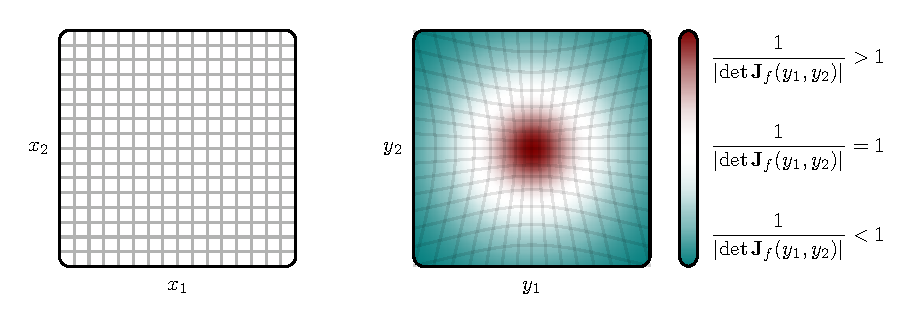
\includegraphics[width=0.8\textwidth,height=\textheight]{figures/warping/warping.pdf}

}

\caption{\label{fig-warping}The reciprocal of the absolute value of the
Jacobian determinant function,
\(1 / \mathrm{det} \, \mathbf{J}_{f}(f^{-1}(y))\) quantifies how warped
the input Lebesgue measure appears relative to the output Lebesgue
measure. If the warping factor is smaller than one then the input
volumes appear to expand and if the warping factor is larger than one
then the input volumes appear to contract.}

\end{figure}

A nearly universal convention in applied probability theory ignores the
fact that this relationship has to hold for only \(\lambda_{Y}\)-almost
all \(y \in Y\) and just takes the warping factor to be \[
\frac{ \mathrm{d} f_{*} \lambda_{X} }{ \mathrm{d} \lambda_{Y}}(y)
=
\frac{1}{ | \mathrm{det} \, \mathbf{J}_{f}(f^{-1}(y)) |}.
\] for all output points \(y \in Y\).

With this convention the transformation rule for Lebesgue probability
density functions along bijective transformations becomes
(Figure~\ref{fig-correct-density-pushforward},
Figure~\ref{fig-incorrect-density-pushforward}) \begin{align*}
f_{*} p(y)
&\overset{\lambda_{Y}}{=} p(f^{-1}(y)) \,
\frac{ \mathrm{d} f_{*} \lambda_{X} }{ \mathrm{d} \lambda_{Y}}(y)
\\
&\overset{\lambda_{Y}}{=} p(f^{-1}(y)) \,
\frac{1}{ | \mathrm{det} \, \mathbf{J}_{f}(f^{-1}(y)) | }.
\end{align*}

\begin{figure}

{\centering 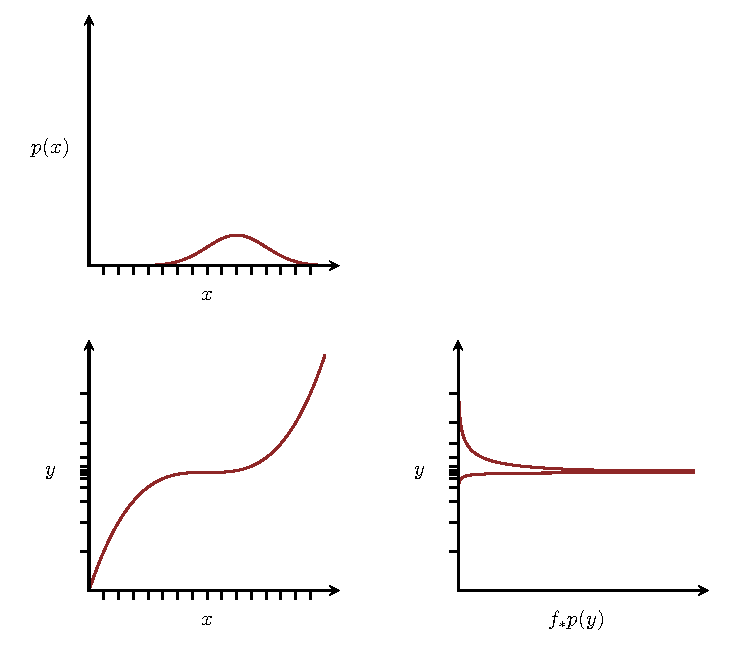
\includegraphics[width=0.75\textwidth,height=\textheight]{figures/pushforwards_density_functions/1d/correct/correct.pdf}

}

\caption{\label{fig-correct-density-pushforward}In general bijective
functions from one real space to another warp both probability
distributions and reference Lebesgue measures. In order to transform
Lebesgue probability density functions we have to account for both of
these changes.}

\end{figure}

\begin{figure}

{\centering 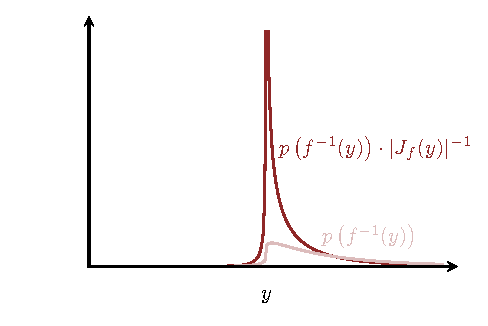
\includegraphics[width=0.5\textwidth,height=\textheight]{figures/pushforwards_density_functions/1d/incorrect/incorrect.pdf}

}

\caption{\label{fig-incorrect-density-pushforward}Ignoring the Jacobian
correction that accounts for the change in Lebesgue reference measure
results in erroneous pushforward probability density functions. This
error affects not only the normalization of the pushforward probability
density function but also its shape.}

\end{figure}

All of this careful work ensures that probability allocations derived
from the pushforward Lebesgue probability density function are
consistent with the probability allocations derived from the initial
Lebesgue probability density function. In particular we always have
(Figure~\ref{fig-integration-consistency}) \begin{align*}
\pi( \mathsf{x} ) &= f_{*} \pi ( f_{*} \mathsf{x} )
\\
\mathbb{E}_{\pi} [ I_{\mathsf{x}} ]
&=
\mathbb{E}_{f_{*} \pi} [ I_{f_{*} \mathsf{x}} ]
\\
\mathbb{I}_{\lambda_{X}} [ p \cdot I_{\mathsf{x}} ]
&=
\mathbb{E}_{\lambda_{Y}} [ f_{*} p \cdot I_{f_{*} \mathsf{x}} ]
\\
\int_{\mathbb{R}^{N}} \mathrm{d}^{N} x \,
p(x) \cdot I_{\mathsf{x}}(x)
&=
\int_{\mathbb{R}^{N}} \mathrm{d}^{N} y \,
f_{*} p(y) \cdot I_{f_{*} \mathsf{x}}(y)
\\
\int_{\mathsf{x}} \mathrm{d}^{N} x \, p(x)
&=
\int_{f_{*} \mathsf{x}} \mathrm{d}^{N} y \, f_{*} p(y).
\end{align*}

\begin{figure}

{\centering 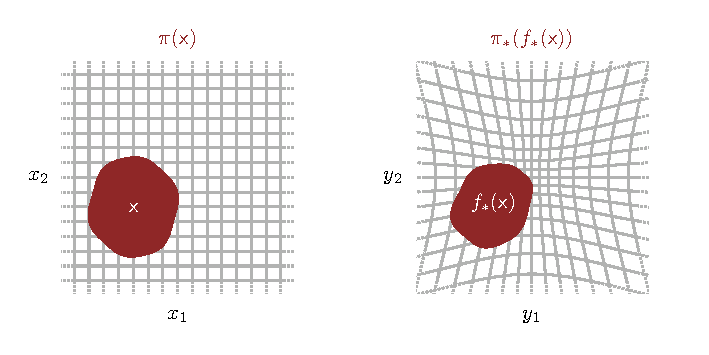
\includegraphics[width=0.8\textwidth,height=\textheight]{figures/integration_consistency/integration_consistency.pdf}

}

\caption{\label{fig-integration-consistency}The proper transformation
rule for Lebesgue probability density functions allows us to
consistently compute probability allocations on the input space and the
output space.}

\end{figure}

When applying the transformation rule for probability density functions
in practice the most common mistake is forgetting the Jacobian
correction entirely. The second most common error is forgetting to take
the reciprocal of the Jacobian determinant, mistakingly using \[
f_{*} p(y)
\overset{\lambda_{Y}}{=}
p(f^{-1}(y)) \, | \mathrm{det} \, \mathbf{J}_{f}(f^{-1}(y)) |.
\] To avoid this mistake I rely on a mneumonic to help me remember the
proper orientation of the Jacobian determinant. I start with the
informal integral relationship, \[
\int \mathrm{d} y \, f_{*} p(y) = \int \mathrm{d} x \, p(x),
\] drop the integral signs, \[
\mathrm{d} y \, f_{*} p(y) = \mathrm{d} x \, p(x),
\] and then very informally divide by the differentials, \begin{align*}
\mathrm{d} y \, f_{*} p(y) &= \mathrm{d} x \, p(x)
\\
f_{*} p(y)
&=
p(x) \, \frac{ \mathrm{d} x }{ \mathrm{d} y } (x)
\\
f_{*} p(y)
&=
p(x(y)) \, \frac{1}{ \frac{ \mathrm{d} y }{ \mathrm{d} x }(x) }
\\
f_{*} p(y)
&=
p(x) \, \frac{1}{ | \mathrm{det} \, \mathbf{J}_{f}(x) |}
\\
f_{*} p(y)
&=
p(f^{-1}(y)) \, \frac{1}{ | \mathrm{det} \, \mathbf{J}_{f}(f^{-1}(y)) |}.
\end{align*} This is by no means a formal calculation -- each step is
extremely mathematically sloppy -- but the result is quick to derive and
gives the correct orientation of the Jacobian correction.

Is there anything we can do about non-bijective functions? We might be
tempted to utilize the Dirac delta function to try to define interated
expectation values on the input space, \begin{align*}
\int_{X} \mathrm{d} x \, \pi(x) \, g(f(x))
&=
\int_{Y} \mathrm{d} y
\left[ \int_{f^{-1}(y)} \mathrm{d} x \, \pi(x) \right] g(y)
\\
&=
\int_{Y} \mathrm{d} y
\left[ \int_{X} \mathrm{d} x \, \pi(x) \delta( f(x) - y ) \right] g(y)
\end{align*} so that \[
f_{*} \pi(y) \overset{\lambda_{Y}}{=}
\int_{X} \mathrm{d} x \, \pi(x) \delta( f(x) - y ),
\] and indeed this notation is not uncommon in some applied fields.

Unfortunately it's not clear how we can actually implement these
constrainted integrals in practice. In the next chapter we'll see how we
can formalize this strategy using \emph{conditional} expectation values
to implement integrals over level sets.

\hypertarget{examples}{%
\subsubsection{Examples}\label{examples}}

After all of that discussion let's put these results in practice with a
few concrete examples.

\hypertarget{translating-and-scaling}{%
\paragraph{Translating and Scaling}\label{translating-and-scaling}}

Consider a probability distribution over a rigid real line, or a fixed
parameterization of a flexible real line, specified by a normal
probability density function \[
\mathrm{normal}(x; \mu, \sigma)
=
\frac{1}{\sqrt{2 \pi} \sigma}
\exp \left(
-\frac{1}{2} \left( \frac{ x - \mu}{\sigma} \right)^{2}
\right).
\]

A translation function maps each point in the input real line to a
translated point in the output real line, \begin{alignat*}{6}
t_{\delta} :\; & \mathbb{R} & &\rightarrow& \; & \mathbb{R} &
\\
& x & &\mapsto& & x + \delta &.
\end{alignat*} This function is a bijection, with the inverse function
translating points in the opposite direction, \begin{alignat*}{6}
t_{\delta}^{-1} :\; & \mathbb{R} & &\rightarrow& \; & \mathbb{R} &
\\
& y & &\mapsto& & y - \delta &.
\end{alignat*}

Because the translation operator maps a one-dimensional space into
another one-dimensional space its Jacobian determinant reduces to a
single derivative function, \begin{align*}
\mathrm{det} \,  \mathbf{J}_{t_{\delta}}(x)
&= \frac{ \mathrm{d} t_{\delta} }{ \mathrm{d} x }(x)
\\
&= \frac{ \mathrm{d} }{ \mathrm{d} x } ( x + \delta )
\\
&= 1.
\end{align*} Consequently the Jacobian correction is particularly
straightforward, \[
\frac{1}
{| \mathrm{det} \, \mathbf{J}_{t_{\delta}}(t_{\delta}^{-1}(y)) |}
=
\frac{1}{ | 1 | }
=
1.
\]

With the Jacobian correction in hand the pushforward of a normal density
function along a translation operator becomes \begin{align*}
(t_{\delta})_{*} \mathrm{normal}(y; \mu, \sigma)
&=
\mathrm{normal}(t_{\delta}^{-1}(y); \mu, \sigma))
\cdot
\frac{1}
{| \mathrm{det} \,  \mathbf{J}_{t_{\delta}}(t_{\delta}^{-1}(y)) |}
\\
&=
\mathrm{normal}(y - \delta; \mu, \sigma) \cdot 1
\\
&= \frac{1}{\sqrt{2 \pi} \sigma}
\exp \left(
-\frac{1}{2} \left( \frac{ y - \delta - \mu}{\sigma} \right)^{2} \right)
\\
&= \frac{1}{\sqrt{2 \pi} \sigma}
\exp \left(
-\frac{1}{2} \left( \frac{ y - (\mu + \delta)}{\sigma} \right)^{2}
\right)
\\
&=
\mathrm{normal}(y; \mu + \delta, \sigma).
\end{align*} In other words pushing a normal probability density
function along a translation operator results in another normal
probability density function, only one with a shifted location parameter
(Figure~\ref{fig-translation}).

\begin{figure}

{\centering 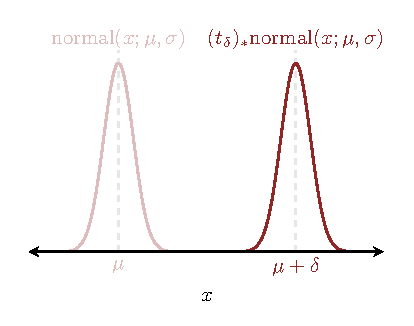
\includegraphics[width=0.6\textwidth,height=\textheight]{figures/pushforwards_density_functions/translation/translation.pdf}

}

\caption{\label{fig-translation}A translation operator \(t_{\delta}\)
shifts a normal probability density function with location parameter
\(\mu\) to another normal probability density function with location
parameter \(\mu + \delta\). The scale parameter \(\sigma\) is
unaffected.}

\end{figure}

A scale function maps each point in the input space to a scaled point in
the output space, \begin{alignat*}{6}
s_{\phi} :\; & \mathbb{R} & &\rightarrow& \; & \mathbb{R} &
\\
& x & &\mapsto& & \phi \cdot x &
\end{alignat*} for any \(\phi > 0\). This is also a bijection, with the
inverse function scaling points by the reciprocal of \(\phi\),
\begin{alignat*}{6}
s_{\phi}^{-1} :\; & \mathbb{R} & &\rightarrow& \; & \mathbb{R} &
\\
& y & &\mapsto& & \frac{y}{\phi} &.
\end{alignat*}

The Jacobian determinant once again reduces to just a single derivative
function, \begin{align*}
\mathrm{det} \, \mathbf{J}_{s_{\phi}}(x)
&= \frac{ \mathrm{d} s_{\phi} }{ \mathrm{d} x }(x)
\\
&= \frac{ \mathrm{d} }{ \mathrm{d} x } ( \phi \cdot x )
\\
&= \phi
\end{align*} In this case the Jacobian correction is slightly more
complicated, \[
\frac{1}{| \mathrm{det} \, \mathbf{J}_{s_{\phi}}(s_{\phi}^{-1}(y)) |}
=
\frac{1}{ | \phi | }
=
\frac{1}{ \phi }.
\]

The pushforward of a normal density function along a scale function is
then given by \begin{align*}
(s_{\phi})_{*} \mathrm{normal}(y; \mu, \sigma)
&=
\mathrm{normal}(s_{\phi}^{-1}(y); \mu, \sigma))
\cdot
\frac{1}{| \mathrm{det} \, \mathbf{J}_{s_{\phi}}(s_{\phi}^{-1}(y)) |}
\\
&=
\mathrm{normal}( y / \phi; \mu, \sigma) \frac{1}{\phi}
\\
&= \frac{1}{\sqrt{2 \pi} \sigma} \cdot \frac{1}{\phi} \,
\exp \left(
-\frac{1}{2} \left( \frac{ y / \phi - \mu}{\sigma} \right)^{2} \right)
\\
&= \frac{1}{\sqrt{2 \pi} (\phi \cdot \sigma)}
\exp \left(
-\frac{1}{2}
\left( \frac{ y - \phi \cdot \mu}{\phi \cdot \sigma} \right)^{2}
\right)
\\
&=
\mathrm{normal}(y; \phi \cdot \mu, \phi \cdot \sigma).
\end{align*} As before pushing a normal probability density function
along a scale operator results in another normal probability density
function. In this case, however, both the location and scale parameters
are affected (Figure~\ref{fig-scale}).

\begin{figure}

{\centering 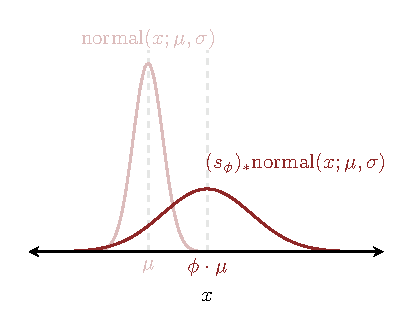
\includegraphics[width=0.6\textwidth,height=\textheight]{figures/pushforwards_density_functions/scale/scale.pdf}

}

\caption{\label{fig-scale}A scale operator \(s_{\phi}\) transforms a
normal probability density function with location parameter \(\mu\) and
scale parameter \(\sigma\) into normal probability density function with
the inflated location parameter \(\phi \cdot \mu\) and inflated scale
parameter \(\phi \cdot \sigma\).}

\end{figure}

These two operations can also be combined into a single function that
first scales and then translates, \[
st_{\delta, \phi} = t_{\delta} \circ s_{\phi}
\] with \begin{alignat*}{6}
st_{\delta, \phi} :\; & \mathbb{R} & &\rightarrow& \; & \mathbb{R} &
\\
& x & &\mapsto& & \phi \cdot x + \delta &.
\end{alignat*} This composition defines another bijection, with the
inverse function scaling points by the reciprocal of the scaling
parameter before translating in the opposite direction, \[
st_{\delta, \phi}^{-1} = s_{\phi}^{-1} \circ t_{\delta}^{-1}
\] with \begin{alignat*}{6}
st_{\delta, \phi}^{-1} :\; & \mathbb{R} & &\rightarrow& \; & \mathbb{R} &
\\
& y & &\mapsto& & \frac{y - \delta}{\phi}  &.
\end{alignat*}

The Jacobian determinant for this composition is \begin{align*}
\mathrm{det} \, \mathbf{J}_{st_{\delta, \phi}}(x)
&= \frac{ \mathrm{d} st_{\delta, \phi} }{ \mathrm{d} x }(x)
\\
&= \frac{ \mathrm{d} }{ \mathrm{d} x } ( \phi \cdot x + \delta )
\\
&= \phi,
\end{align*} with the Jacobian correction becoming \[
\frac{1}
{| \mathrm{det} \, \mathbf{J}_{st_{\delta, \phi}}
(st_{\delta, \phi}^{-1}(y)) |}
=
\frac{1}{ | \phi | }
=
\frac{1}{ \phi }.
\]

Pushing forward a normal probability density function along this
composite function then gives \begin{align*}
(st_{\delta, \phi})_{*} \mathrm{normal}(y; \mu, \sigma)
&=
\mathrm{normal}(st_{\delta, \phi}^{-1}(y); \mu, \sigma)
\cdot
\frac{1}
{| \mathrm{det} \, \mathbf{J}_{st_{\delta, \phi}}(s_{\phi}^{-1}(y)) |}
\\
&=
\mathrm{normal}( (y - \delta) / \phi ; \mu, \sigma) \cdot (1 / \phi)
\\
&= \frac{1}{\sqrt{2 \pi} \sigma} \frac{1}{ \phi }
\exp \left(
-\frac{1}{2}
\left( \frac{ (y - \delta) / \phi - \mu}{\sigma} \right)^{2}
\right)
\\
&= \frac{1}{\sqrt{2 \pi} (\phi \cdot \sigma)}
\exp \left(
-\frac{1}{2}
\left(
\frac{ y - (\phi \cdot \mu + \delta)}{\phi \cdot \sigma}
\right)^{2}
\right)
\\
&=
\mathrm{normal}(y; \phi \cdot \mu + \delta, \phi \cdot \sigma).
\end{align*} No matter how we scale and translate an ambient real line,
a normal probability density function will always map into another
normal probability density function.

In fact if we start with the \textbf{unit normal probability density
function} \[
\text{unit-normal}(x) = \text{normal}(x; 0, 1),
\] then the pushforward probability density function along the
scale-translation function becomes \[
(st_{\delta, \phi})_{*} \text{unit-normal}(y)
=
\mathrm{normal}(y; \delta, \phi).
\] Consequently we can generate \emph{every} normal probability density
function as a suitable transformation of an initial, unit normal
probability density function. Because of this the normal family of
probability density functions is known as a \textbf{location-scale}
family.

\hypertarget{squeezing-a-real-line-into-an-interval}{%
\paragraph{Squeezing A Real Line Into An
Interval}\label{squeezing-a-real-line-into-an-interval}}

For a more sophisticated example let's look at the logistic function
that we introduced in \href{@sec:terminology}{Section 2.1},
\begin{alignat*}{6}
\text{logistic} :\; & \mathbb{R} & &\rightarrow& \; & (0, 1) &
\\
& x & &\mapsto& & \frac{1}{1 + \exp(-x)} &.
\end{alignat*} The logistic function is bijective and its inverse
function is known as the \textbf{logit function}, \begin{alignat*}{6}
\text{logit} :\; & (0, 1) & &\rightarrow& \; & \mathbb{R} &
\\
& y & &\mapsto& & \log \frac{y}{1 - y} &.
\end{alignat*}

Because this is a one-dimensional transformation the Jacobian
determinant reduces to a single derivative function, \begin{align*}
\mathrm{det} \, \mathbf{J}_{\text{logistic}}(x)
&=
\frac{ \mathrm{d} \text{logistic} }{ \mathrm{d} x }(x)
\\
&=
\frac{ \mathrm{d} }{ \mathrm{d} x } \left( \frac{1}{1 + \exp(-x)} \right)
\\
&=
- \frac{\exp(-x)}{(1 + \exp(-x))^{2}}
\\
&=
- \frac{1}{1 + \exp(-x)} \left(1 - \frac{1}{1 + \exp(-x)} \right)
\\
&=
- \text{logistic}(x) \left(1 - \text{logistic}(x) \right).
\end{align*} The Jacobian correction then becomes \begin{align*}
\frac{1}{| \mathrm{det} \, \mathbf{J}_{\text{logistic}}(\text{logit}(y)) |}
&=
\frac{1}{ | - \text{logistic}(\text{logit}(y))
              \left(1 - \text{logistic}(\text{logit}(y)) \right) | }
\\
&=
\frac{1}{ \text{logistic}(\text{logit}(y))
          \left(1 - \text{logistic}(\text{logit}(y)) \right) }
\\
&=
\frac{1}{ y \left(1 - y \right) }.
\end{align*}

The pushforward of a normal density function along the logistic function
is now given by (Figure~\ref{fig-logistic}) \begin{align*}
\text{logistic}_{*} \mathrm{normal}(y; \mu, \sigma)
&=
\mathrm{normal}( \text{logit}(y); \mu, \sigma)
\cdot \frac{1}{| \mathrm{det} \, \mathbf{J}_{\text{logistic}}(\text{logit}(y)) |}
\\
&=
\mathrm{normal}( \text{logit}(y); \mu, \sigma) \frac{1}{y(1 - y)}.
\end{align*}

\begin{figure}

{\centering 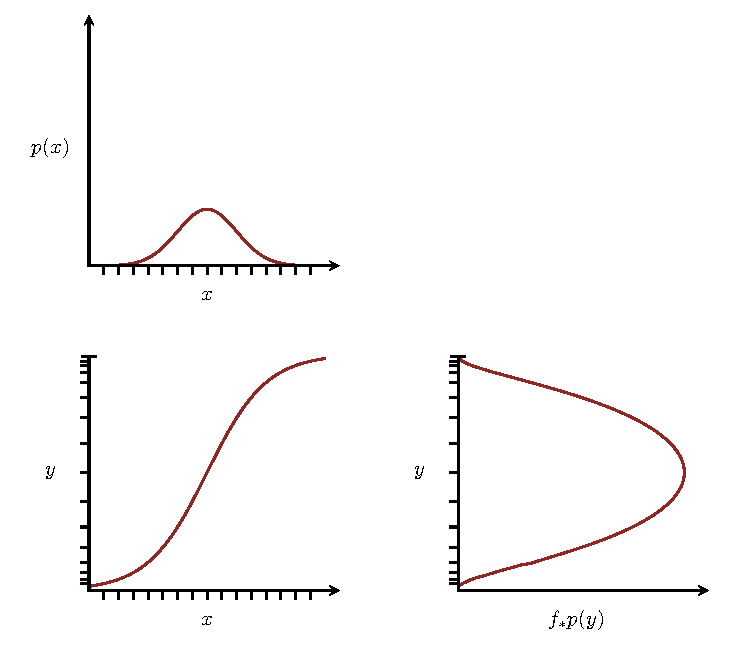
\includegraphics[width=0.75\textwidth,height=\textheight]{figures/pushforwards_density_functions/logistic/logistic.pdf}

}

\caption{\label{fig-logistic}The logistic function squeezes a real line
into a unit interval, transforming Lebesgue probability density
functions over all real numbers into a Lebesgue probability density
function over real numbers \(0 < y < 1\).}

\end{figure}

\hypertarget{sec:1d-pushforward-characterizations}{%
\section{Characterizing One-Dimensional Pushforward Probability
Distributions}\label{sec:1d-pushforward-characterizations}}

Probability distributions on high-dimensional spaces are overwhemlming
objects that are difficult to study directly. In particular we cannot
convey the entirety of a high-dimensional probability distribution in a
single visualization. We can, however, push a high-dimensional
probability distribution forward to many one-dimensional probability
distributions that can be visualized
(Figure~\ref{fig-projective-viewing}), not unlike a carpenter checking
if a piece of wood is warped by staring down each edge one at a time.

\begin{figure}

\begin{minipage}[t]{0.25\linewidth}

{\centering 

~

}

\end{minipage}%
%
\begin{minipage}[t]{0.50\linewidth}

{\centering 

\raisebox{-\height}{

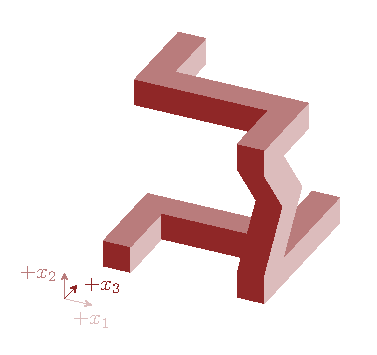
\includegraphics{figures/projective_viewing/uninformative_perspective/uninformative_perspective.pdf}

}

}

\subcaption{\label{fig-uninformative-perspective}}
\end{minipage}%
%
\begin{minipage}[t]{0.25\linewidth}

{\centering 

~

}

\end{minipage}%
\newline
\begin{minipage}[t]{0.05\linewidth}

{\centering 

~

}

\end{minipage}%
%
\begin{minipage}[t]{0.90\linewidth}

{\centering 

\raisebox{-\height}{

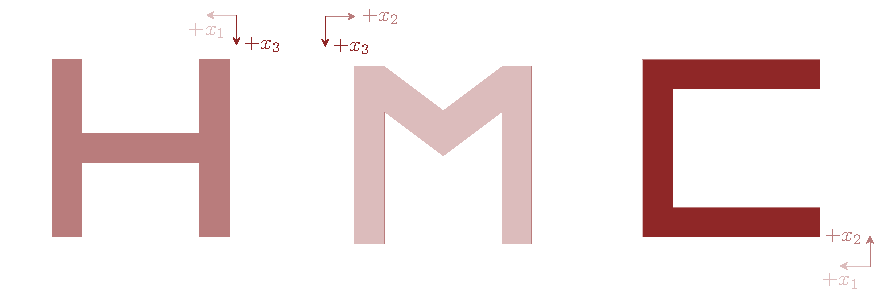
\includegraphics{figures/projective_viewing/informative_perspectives/informative_perspectives.pdf}

}

}

\subcaption{\label{fig-informative-perspectives}}
\end{minipage}%
%
\begin{minipage}[t]{0.05\linewidth}

{\centering 

~

}

\end{minipage}%

\caption{\label{fig-projective-viewing}In general (a) High-dimensional
mathematical objects, such probability distributions over
high-dimensional spaces, are difficult to interpret directly. (b)
Summary functions map high-dimensional objects to low-dimensional
objects, isolating behaviors that can be not only easier to digest but
also straightforward to visualize.}

\end{figure}

More formally given a probability space \((X, \mathcal{X}, \pi)\) and a
collection of measurable functions \[
f_{n} : (X, \mathcal{X}) \rightarrow
        (\mathbb{R}, \mathcal{B}_{\mathbb{R}})
\] we can construct a collection of one-dimensional pushforward
probability distributions \[
(f_{n})_{*} \pi.
\] Each of these pushforward probability distributions summarizes a
different aspect of \(\pi\); the more interpretable the outputs of the
function \(f_{n}\) are the more interpretable that summary will be.

In order to implementing these probabilistic summaries in practice,
however, we need to be able to characterize the pushforward probability
distributions. Pushforward probability density functions would be
particularly convenient for visualization
(Figure~\ref{fig-pushforward-characterizations-density}), but at this
point we don't know how to actually compute them yet for non-bijective
summary functions. Unfortunately in the next chapter we'll see that the
necessary operations are often infeasible in practice.

\begin{figure}

{\centering 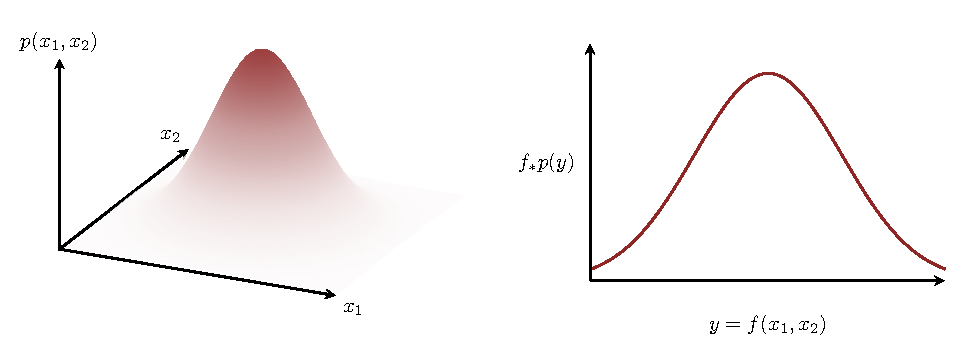
\includegraphics[width=0.8\textwidth,height=\textheight]{figures/pushforward_characterizations/density/density.pdf}

}

\caption{\label{fig-pushforward-characterizations-density}A pushforward
probability density functions are particularly useful for visualizing
pushforward behavior extracted from a high-dimensional probability
distribution, but they often infeasible to construct in practice.}

\end{figure}

Fortunately in
\href{https://betanalpha.github.io/assets/chapters_html/expectation_values.html}{Chapter
Five} we learned about multiple ways to characterize one-dimensional
probability distributions using only expectation values. Moreover if we
can compute expectation values on the initial, high-dimensional ambient
space then we can use the pullback of expectation values, \[
\mathbb{E}_{f_{*} \pi}[ g ] = \mathbb{E}_{\pi} [ g \circ f ].
\] to implement these characterizations in practice.

For example in \href{@sec:transforming-integrals}{Section 3} we saw that
the moments of one-dimensional pushforward distributions can be
evaluated as expectation values over the initial space. In particular we
can compute the mean and variance of the pushfoward probability
distribution \((f_{n})_{*} \pi\) can be evaluated with the expectation
values \[
\mathbb{M}_{(f_{n})_{*} \pi}
=
\mathbb{E}_{\pi} [ f_{n} ]
\] and \[
\mathbb{V}_{f^{*} \mu}
=
\mathbb{E}_{(f_{n})_{*} \pi} [ (f - \mathbb{M}_{(f_{n})_{*} \pi})^{2} ],
\] respectively. That is, of course, provided that both expectands are
integrable.

We can also use expectation values to evaluate pushforward interval
probabilities, \begin{align*}
(f_{n})_{*} \pi( \, (y_{1}, y_{2} ] \, )
&=
\mathbb{E}_{(f_{n})_{*} \pi} \left[ I_{(y_{1}, y_{2} ]} \right]
\\
&=
\mathbb{E}_{\pi} \left[ I_{(y_{1}, y_{2} ]} \circ f_{n} \right].
\end{align*}

These pushforward interval probabilities then allow us to construct
histogram representations of each pushforward probability distribution
(Figure~\ref{fig-pushforward-characterizations-histogram}). The narrower
the pushforward intervals we use the more these histograms convey the
same information that a pushforward probability density function would,
especially when we scale the bin probabilities by the interval lengths
as we discussed in
\href{https://betanalpha.github.io/assets/chapters_html/density_functions.html\#lebesgue-probability-densities-as-limiting-interval-probabilities}{Chapter
Six, Section 4.4}.

\begin{figure}

{\centering 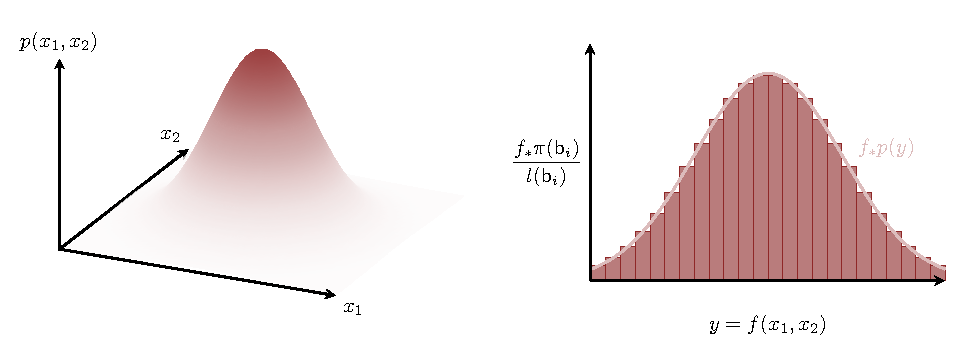
\includegraphics[width=0.8\textwidth,height=\textheight]{figures/pushforward_characterizations/histogram/histogram.pdf}

}

\caption{\label{fig-pushforward-characterizations-histogram}Pushforward
histograms visualize similar information as pushforward probability
density functions, especially when the binning is narrow, but are much
easier to construct.}

\end{figure}

In theory we can also use pushforward interval probabilities to
construct the cumulative distribution functions for a given pushforward
probability distribution by computing \begin{align*}
P_{f_{*} \pi}(y)
&=
(f_{n})_{*} \pi( \, (-\infty, y] \, )
\\
&=
\mathbb{E}_{\pi} \left[ I_{(-\infty, y]} \circ f_{n} \right]
\end{align*} for each \(y \in \mathbb{R}\). Unfortunately completely
characterizing a pushforward cumulative distribution function in this
way would require an infinite number of expectation value calculations
while typical computational budgets afford for only a finite number.
Consequently in practice we have to be content with \emph{approximating}
pushforward cumulative distribution functions
(Figure~\ref{fig-pushforward-characterizations-cdf}).

\begin{figure}

{\centering 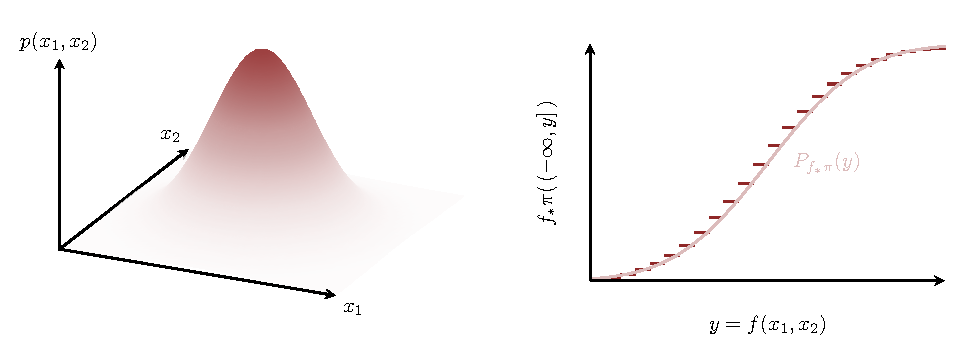
\includegraphics[width=0.8\textwidth,height=\textheight]{figures/pushforward_characterizations/cdf/cdf.pdf}

}

\caption{\label{fig-pushforward-characterizations-cdf}Aggregating bin
probabilities also allows us to approximately visualize a pushforward
cumualtive distribution function.}

\end{figure}

Lastly we can often characterize one-dimensional pushforward probability
distribution with nested pushforward quantile intervals
(Figure~\ref{fig-pushforward-characterizations-quantile-intervals}).
While we typically won't be able to compute pushforward quantiles
exactly, we can construct reasonable approximations to the \(p\)-th
quantile by iteratively searching possible values
\(q_{p} \in \mathbb{R}\) until \[
| (f_{n})_{*} \pi( \, (-\infty, q_{p}] \, ) - p |
=
| \mathbb{E}_{\pi} \left[ I_{(-\infty, y]} \circ f_{n} \right] - p |
\] is sufficiently small.

\begin{figure}

{\centering 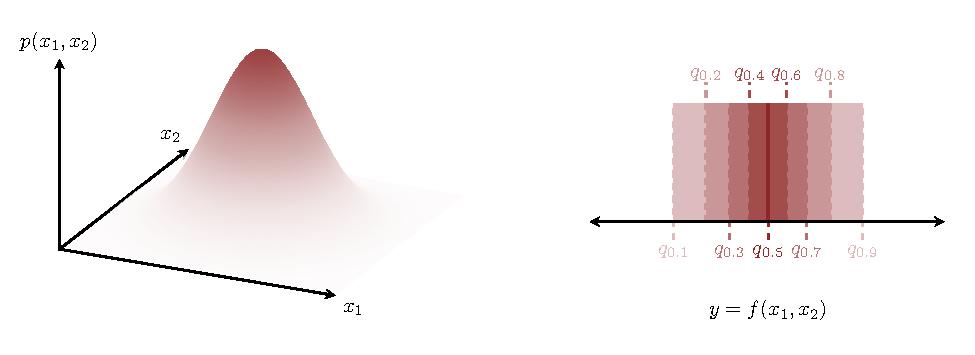
\includegraphics[width=0.8\textwidth,height=\textheight]{figures/pushforward_characterizations/quantile_intervals/quantile_intervals.pdf}

}

\caption{\label{fig-pushforward-characterizations-quantile-intervals}Nested
quantile intervals provide a compact characterization of one-dimensional
pushforward distributions.}

\end{figure}

I personally find histogram characterizations to be the most robust
compromise between practical feasibility and visual information density,
and we will be using them often in this book. Because they can be
condensed into a single line nested quantile intervals can also be
convenient when visualizing many pushforward distributions at the same
time (Figure~\ref{fig-quantile-ribbons}). These visualizations are also
know as \textbf{fan plots} or \textbf{ribbon plots}.

\begin{figure}

\begin{minipage}[t]{0.05\linewidth}

{\centering 

~

}

\end{minipage}%
%
\begin{minipage}[t]{0.45\linewidth}

{\centering 

\raisebox{-\height}{

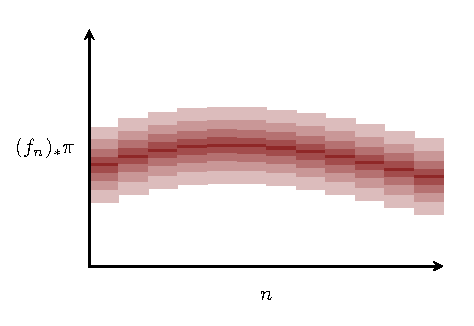
\includegraphics{figures/pushforward_characterizations/quantile_ribbons/discrete/discrete.pdf}

}

}

\subcaption{\label{fig-discrete-quantile-ribbons}}
\end{minipage}%
%
\begin{minipage}[t]{0.45\linewidth}

{\centering 

\raisebox{-\height}{

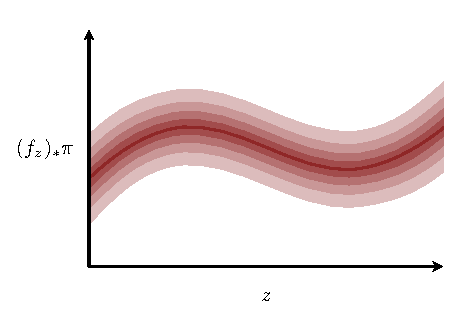
\includegraphics{figures/pushforward_characterizations/quantile_ribbons/continuous/continuous.pdf}

}

}

\subcaption{\label{fig-continuous-quantile-ribbons}}
\end{minipage}%
%
\begin{minipage}[t]{0.05\linewidth}

{\centering 

~

}

\end{minipage}%

\caption{\label{fig-quantile-ribbons}Nested quantile intervals are
particularly useful for visualizing both (a) finite collections of
summary functions that can be indexed by integers \(n \in \mathbb{Z}\)
and (b) uncountably infinite collections of summary functions that can
be indexed by real numbers \(z \in \mathbb{R}\). These visualizations
are somewhat limited because they don't convey the correlations between
the summary function outputs but with that caveat in mind they can be
incredibly effective.}

\end{figure}

\hypertarget{conclusion}{%
\section{Conclusion}\label{conclusion}}

The ability to transform probabilistic objects, in particular the
ability to actually implement these transformations in practice, is an
extremely powerful tool in applied probability theory. These
transformations allow us to not only manipulate probability spaces into
more convenient forms but also distill high-dimensional probabilistic
information to low-dimensional summary spaces that are straightforward
to visualize.

\hypertarget{acknowledgements}{%
\section*{Acknowledgements}\label{acknowledgements}}
\addcontentsline{toc}{section}{Acknowledgements}

A very special thanks to everyone supporting me on Patreon: Adam
Fleischhacker, Adriano Yoshino, Alan Chang, Alessandro Varacca,
Alexander Noll, Alexander Petrov, Alexander Rosteck, Andrea Serafino,
Andrew Mascioli, Andrew Rouillard, Andrew Vigotsky, Angie\_Hyunji Moon,
Ara Winter, Austin Rochford, Austin Rochford, Avraham Adler, Ben
Matthews, Ben Swallow, Benoit Essiambre, Bradley Kolb, Brandon Liu,
Brendan Galdo, Brynjolfur Gauti Jónsson, Cameron Smith, Canaan Breiss,
Cat Shark, Charles Naylor, Chase Dwelle, Chris, Chris Jones, Christopher
Cahill, Christopher Mehrvarzi, Colin Carroll, Colin McAuliffe, Damien
Mannion, Damon Bayer, dan mackinlay, Dan W Joyce, Dan Waxman, Dan
Weitzenfeld, Daniel Edward Marthaler, Darshan Pandit, Darthmaluus ,
David Galley, David Wurtz, Denis Vlašiček, Doug Rivers, Dr.~Jobo,
Dr.~Omri Har Shemesh, Dylan Maher, Ed Cashin, Edgar Merkle, Eric
LaMotte, Ero Carrera, Eugene O'Friel, Felipe González, Fergus Chadwick,
Finn Lindgren, Florian Wellmann, Francesco Corona, Geoff Rollins, Guido
Biele, Hamed Bastan-Hagh, Haonan Zhu, Hector Munoz, Henri Wallen, herr,
hs, Hugo Botha, Håkan Johansson, Ian, Ian Costley, idontgetoutmuch,
Ignacio Vera, Ilaria Prosdocimi, Isaac Vock, J, J Michael Burgess, Jair
Andrade, James C, James Hodgson, James Wade, Janek Berger, Jason Martin,
Jason Pekos, Jason Wong, Jeff Burnett, Jeff Dotson, Jeff Helzner,
Jeffrey Erlich, Jesse Wolfhagen, Jessica Graves, Joe Wagner, John
Flournoy, Jonathan H. Morgan, Jonathon Vallejo, Joran Jongerling, Joshua
Griffith, JU, Justin Bois, Karim Naguib, Karim Osman, Kejia Shi,
Kristian Gårdhus Wichmann, Kádár András, Lars Barquist, lizzie , LOU
ODETTE, Luís F, Marcel Lüthi, Marek Kwiatkowski, Mark Donoghoe, Markus
P., Martin Modrák, Matt Moores, Matthew, Matthew Kay, Matthieu LEROY,
Mattia Arsendi, Maurits van der Meer, Michael Colaresi, Michael DeWitt,
Michael Dillon, Michael Lerner, Mick Cooney, Márton Vaitkus, N Sanders,
N.S. , Name, Nathaniel Burbank, Nic Fishman, Nicholas Clark, Nicholas
Cowie, Nick S, Octavio Medina, Oliver Crook, Olivier Ma, Patrick Kelley,
Patrick Boehnke, Pau Pereira Batlle, Pieter van den Berg , ptr, Ramiro
Barrantes Reynolds, Ravin Kumar, Raúl Peralta Lozada, Riccardo Fusaroli,
Richard Nerland, Robert Frost, Robert Goldman, Robert kohn, Robin
Taylor, Ryan Grossman, Rémi , S Hong, Scott Block, Sean Pinkney, Sean
Wilson, Sergiy Protsiv, Seth Axen, shira, Simon Duane, Simon Lilburn,
sssz, Stan\_user, Stephanie Fitzgerald, Stephen Lienhard, Steve
Bertolani, Stew Watts, Stone Chen, Susan Holmes, Svilup, Tao Ye, Tate
Tunstall, Tatsuo Okubo, Teresa Ortiz, Theodore Dasher, Thomas Vladeck,
Tiago Cabaço, Tim Radtke, Tobychev , Tom McEwen, Tomáš Frýda, Tony
Wuersch, Virginia Fisher, Vitaly Druker, Vladimir Markov, Wil Yegelwel,
Will Farr, Will Tudor-Evans, woejozney, yolhaj , Zach A, Zad Rafi, and
Zhengchen Ca.

\hypertarget{references}{%
\section*{References}\label{references}}
\addcontentsline{toc}{section}{References}

\hypertarget{refs}{}
\begin{CSLReferences}{1}{0}
\leavevmode\vadjust pre{\hypertarget{ref-Apostol:1969}{}}%
Apostol, Tom M. 1969. \emph{Calculus. {V}ol. {II}: {M}ulti-Variable
Calculus and Linear Algebra, with Applications to Differential Equations
and Probability}. Second. Blaisdell Publishing Co. {[}Ginn; Co.{]},
Waltham, Mass.-Toronto, Ont.-London.

\leavevmode\vadjust pre{\hypertarget{ref-Folland:1999}{}}%
Folland, G. B. 1999. \emph{Real Analysis: Modern Techniques and Their
Applications}. New York: John Wiley; Sons, Inc.

\end{CSLReferences}

\hypertarget{license}{%
\section*{License}\label{license}}
\addcontentsline{toc}{section}{License}

A repository containing all of the files used to generate this chapter
is available on
\href{https://github.com/betanalpha/quarto_chapters/tree/main/7_transforming_probability_spaces}{GitHub}.

The text and figures in this chapter are copyrighted by Michael
Betancourt and licensed under the CC BY-NC 4.0 license:

https://creativecommons.org/licenses/by-nc/4.0/



\end{document}
